% !TeX root=../main.tex



\section{Probabilistic Trace Alignment Pipeline}
Our approach takes as input
\begin{inparaenum}[\it (i)]
\item a reference model represented as an \uswn $\net$,
\item a minimum, positive probability threshold $\pmin \in (0,1]$
\item a trace $\trace$ of interest,
\end{inparaenum}
and returns a ranking over all the $\net$-traces having a probability $\geq\pmin$, combining their probability values (probabilistic component) and their distance to $\trace$ (alignment component).



\subsection{Computation pipeline}
The approach is realized through the pipeline shown in \figurename~\ref{fig:pipe}, consisting of the following five steps.
%
In step 1, the reachability graph $\rg{\net}$ of $\net$ is constructed.
%
In step 2,  $\rg{\net}$ is converted into a corresponding transition graph $\tg_{\rg{\net}}$ that preserves model traces and their probabilities. We omit the details of this conversion, due to lack of space and the fact that it employs well-known techniques used to \emph{shift labels} from transitions to states while preserving the behavior encoded by a transition system. \figurename~\ref{fig:orig} shows the result of this conversion when applied to the reachability graph in \figurename~\ref{fig:rg}.


In step 3, the transition graph $\tg_{\rg{\net}}$ is processed applying a \emph{$\hidden$-closure } that compiles away
$\tau$-transitions. This results into a new transition graph $\closed{\tg_{\rg{\net}}}$ that retains $\hidden$ labels only in the initial and accepting states and for the rest exclusively employs visible labels in $\tasks$, while preserving model traces and their probabilities. Also in this case we omit the details: the transformation relies on well-known automata-based techniques for removing $\epsilon$-moves. The only non-trivial observation is that, even in our case where probabilities are present, all $\tau$ transitions can still be removed thanks to the working hypothesis done for \uswn{s} in Sect.~\ref{subsec:spn}, namely absence of fully silent loops. As a result of this step, the transition graph in \figurename~\ref{fig:orig} results in that of \figurename~\ref{fig:closed}.


In step 4, the $\hidden$-closed transition graph $\closed{\tg_{\rg{\net}}}$ is \unravelled, so as to collect all the model traces that have a probability of at least $\pmin$. To do so, we rely on the properties in Remarks 2 and 3 from Sect.~\ref{sec:pns}, which are inherited by $\closed{\tg_{\rg{\net}}}$. Specifically, they imply that no loop can be executed without strictly decreasing the resulting probability. This means that all valid sequences with a resulting probability of at least $\pmin$ can be enumerated and returned in a set. The so-obtained sequences are combined by merging those that produce the same trace, summing up their probabilities, thus obtaining the set $\ptraces{\closed{\tg_{\rg{\net}}}}{\pmin}$ of all the traces with probability $\geq \pmin$. The closure operation also implies that the notion of model trace coincides with that of run, modulo removing the two $\tau$ labels attached to the initial and accepting nodes.


%$\closed{\tg_{\rg{\net}}}$ preserves model traces and their probabilities while working only over visible tasks in $\tasks$;
% this transition graph is unraveled c we apply a probabilistic alignment technique that ranks all such model traces according to their probability and their similarity to $\trace$.
%
%The pipeline has the following phases: after representing the USWN as a graph of all the sequentially scheduled transitions
%(Sect.\ref{sec:seqZ}), we shift the labels from the edges towards the nodes while preserving the set of probabilistic traces
%(Sect.\ref{sec:LSift}) and minimize the graph representation by removing the $\tau$-labeled nodes while preserving the
%trace probability (Sect.\ref{sec:clos}).
The last step takes the so-obtained model traces and ranks them by considering their probabilities and the similarity with the log trace $\trace$ of interest. In \figurename~\ref{fig:pipe}, this is shown as a black-box. As we describe next, we have implemented this last step in two alternative ways: one computationally demanding but guaranteeing an optimal-ranking, the other more efficient but providing approximate ranking without optimality guarantees.
%\todo{Ho tagliato la descrizione che c'era dopo. Al limite la incorporerei nella rispettiva sottosezione.}
%We later discuss how to rank traces in the exact and approximated scenarios by reducing the alignment process to a k-nearest
%neighbour problem. While the exact trace alignment requires to perform the alignment process each time a novel trace $\sigma^*$ is
%introduced (Sect.\ref{subsec:exbkptap}), the approximated alignment can split the alignment into a preliminary loading phase and a
%query phase. In the former, each stochastic trace from the USWN is represented as a vector (Sect.\ref{subsec:ate}), and in the latter the to-be-aligned trace $\sigma^*$ is first represented as a vector and then compared to all the other vectorial representations.



\subsection{Alignment Strategies}\label{subsec:as}
%To compute the probabilistic alignments, we transform an SWN (\figurename \ref{fig:spn}) into the corresponding reachability graph (\figurename \ref{fig:rg}) and the reachability graph into a node-labeled Markovian Process. Traces are aligned with this latter representation of the process since, although model trace probabilities can be directly computed by inspecting the reachability graph, graph embedding techniques required to represent traces as data points (e.g., vectors) cannot directly be defined over reachability graphs \cite{GartnerFW03}.
%, called \textsc{Transition Graph} $TG=(L,R)$, where $L$ is called node-labeling matrix and $R$ transition matrix. Such matrices can determine the probability of reaching a node labeled with $\beta\inSect.igma$ from any node labeled with $\alpha\in\Sigma$ in $n$ steps as in string kernels: $[\Lambda^n]_{\alpha\beta}:=[LR^nL^\top]_{\alpha\beta}/[LL^\top]_{\alpha\alpha}$ (see \cite{GartnerFW03} and Example \ref{ex:wheredotiszero}).
%
%To transform a reachability graph into a node-labeled Markovian Process, first, we need to shift labels from edges to nodes (\figurename \ref{fig:lmc}), and then we perform $\tau$-closures while preserving (if required) $\tau$-transitions for both start and final nodes (\figurename \ref{fig:closed}); such operations preserve the probabilities of model traces \cite{Bergami21}. This Markovian Process is called \textsc{Transition Graph}.

%\begin{definition} A \emph{(Probabilistic) Transition Graph} is a tuple $(V,s,t,L,R)$ where:
%	\begin{inparaenum}[\itshape (i)]
%		\item $V \subset \mathbb{N}$ is a set of \emph{nodes};
%		\item $s\in V$ is the \emph{initial node};
%		\item $e\in V$ is the \emph{accepting node};
%		\item $L: \alphabet \times V \rightarrow \{0,1\}$ is a \emph{label matrix} associating each node in $V$ to a single label in $\alphabet$, where for label $\alpha \in \alphabet$ and node $\ind{i} \in V$, $[L]_{\alpha\ind{i}}$ gives $1$ if $\ind{i}$ is labeled by $\alpha$, $0$ otherwise;
%		\item $R: V \times V \rightarrow [0,1]$ is a \emph{(probabilistic) transition matrix} indicating, for each pair of nodes, what is the probability that executing a transition from the first node leads to the second node.
		% \item $\omega \in [0,1]$ is a \emph{graph weight} indicating an overall value associated to the entire graph.
%	\end{inparaenum}
%	$L$ and $R$ satisfy the following well-formedness conditions:
%	\begin{inparaenum}[\itshape (i)]
%		\item for every $i \in V$ there is one and only one label $\alpha \in \alphabet$ so   that $[L]_{\alpha\ind{i}}=1$;
%		\item  for  every $\ind{i} \in V$, we have that $\sum_{\ind{j}\in V}[R]_{\ind{ij}}=1$.
%	\end{inparaenum}
%\end{definition}
%The condition for $L$ indicates that
%Matrices $L$ and $R$ can be exploited to determine the probability of reaching a node labeled by $\beta\in\Sigma$ from any node labeled $\alpha\in\Sigma$ in $n$ steps with $[LR^n\transp{L}]_{\alpha\beta}/[L\transp{L}]_{\alpha\alpha}$ \cite{GartnerFW03}.
%, that we can shorthand as $[G.\Lambda^n]_{\alpha\beta}$ \cite{GartnerFW03}.
%
%$R$ contains the transition probabilities, while for each node $i$ there is only one label $\alpha$ such that $[L]_{i\alpha}=1$, and $[L]_{i\beta}=0$ if $\alpha\neq\beta$.
%Runs for Markovian Processes are then defined as for SWNs, and we employ the same notation to indicate the valid sequences underlying a model trace. The computation of probabilities for traces is hence defined equivalently.
%We denote these pair of matrices as \textsc{Transition Graph} $TG=(L,R)$.

Upon aligning an event log with a stochastic net, distinct model traces have different probabilities. Hence the retrieval of the best model traces maximizing the combined provision of minimum trace alignment cost and maximum model trace probability might not suffice. In some cases, the user could favor an alignment with a lower cost even if based on a less probable model trace, while, in other cases, they may prefer a model trace with a higher probability at the expense of a higher alignment cost. Hence, we align a log trace with a transition graph by retrieving the best $k$ alignments among all model traces in $\ptraces{\net}{\pmin}$. This reduces to the
$k$NN problem by finding the $k$ nearest data points to a \textit{query} $x$ from a set
$\mathcal{X}$ of \textit{data points} w.r.t.\ a given distance function $d_k$. 
%Through ad-hoc data structures, such as VP-Trees
%and KD-Trees, %VP-Trees \cite{Fu2000} \cite{Maneewongvatana99}, and M-Trees \cite{Ciaccia},
%we can retrieve the $k$-neighborhood of $x$ in $\mathcal{X}$ by pre-ordering (\textit{indexing}) $\mathcal{X}$ with respect to $d_k$.
%and searching from the top-$1$ alignment.
%
%To align a trace $\logtrace$ over the \unravelled\ traces $\ptraces{\tg}{\pmin}$,
%the $k$-Nearest Neighbors describe the best $k$ alignments for $\logtrace$.
%We discuss two strategies to obtain these
%alignments.

\smallskip
\noindent
\textbf{Optimal-Ranking Trace Aligner.}
{Here we reuse existing trace aligners such as \cite{DBLP:conf/edoc/AdriansyahDA11,LeoniM17}, where $d(\logtrace,\nonlogtrace)$ is the Levenshtein distance.
%, i.e., the {minimum} cost for aligning one of the two traces with respect to the other when all the possible moves have cost equal to 1.\footnote{This is slightly different from the Levenshtein distance from the literature since here the replacement is obtained as a concatenation of a deletion and an addition.}
We express the ranking score as the product $\probskip{\nonlogtrace} d(\logtrace,\nonlogtrace)$, considering the cost of the alignment (i.e., the distance between the model trace and the trace to be aligned) and the probability of the model trace.
%
To represent the same intuition of such a weighted distance as a ranking function, we transform it into a
similarity function returning $1$ when $\nonlogtrace=\logtrace$ and $\probskip{\logtrace}=1$ hold. We then express $d$ as}
%\xout{We can express our probabilistic trace alignment as finding the trace that maximizes both the trace's probability and its similarity with the query trace $\logtrace$. Still, the trace alignments problems are usually expressed via trace alignments cost functions, and not via trace similarities \cite{LeoniM17}. Given a generic trace cost function $d(\trace,\trace')$, it is always possible to convert it into}
a normalized similarity score $s_d(\logtrace,\nonlogtrace):=\frac{1}{d(\logtrace,\nonlogtrace)+1}$. The maximum similarity is reached when the distance is $0$ and the similarity decreases while the distance increases. %\xout{As a consequence, the exact trace aligner will find the weighted trace $\braket{\trace,\mathbb{P}(\trace)}$ in $\mathcal{W}_{\pmin}(P)$ maximising $s_d(\trace,\logtrace)$, and use $s_d$ as a ranking function.} \ADD
{The golden ranking function (i.e., the one producing the optimal-ranking) can therefore be represented as $\goldenrank(\logtrace,\nonlogtrace)=\probskip{\nonlogtrace} \probskip{\logtrace} s_d(\logtrace,\nonlogtrace)$. The computation ${\max\arg}_{\nonlogtrace\in \WCal{\pmin}{n}} \goldenrank(\logtrace,{\nonlogtrace})$ returns the best optimal-ranking trace alignment for a log trace $\logtrace$, where $\goldenrank$ must be computed a-new for all the possible $\logtrace$.



\smallskip
\noindent
\textbf{Approximate-Ranking Trace Embedder.}
%\label{subsec:ate}
Ranking optimality comes at the sub-optimal cost of a brute-force recomputation of $\goldenrank$ for each novel trace $\logtrace$ to align.
%\footnote{By embedding  all the \unravelled\ model traces via $\phi_{\logtrace}(\nonlogtrace)=\Big(\frac{1}{\probskip{\nonlogtrace}\sqrt{\probskip{\nonlogtrace}^2+s_d^2(\logtrace,\nonlogtrace)}},\frac{1}{s_d(\logtrace,\nonlogtrace)\sqrt{\probskip{\nonlogtrace}^2+s_d^2(\logtrace,\nonlogtrace)}}\Big)$ over a specific $\logtrace$, by representing  $\logtrace$ as $(0,0)$, and by using the Euclidean Distance as a distance, we ensure that all the neighbors of $(0,0)$ will represent the top-$k$ best alignments for $\logtrace$.}. %This is not optimal for $k$NN-based techniques, as this entails the  redefinition of the multidimensional search space $\mathcal{X}$ for each new alignment $\logtrace$. The ``recomputation cost'' could be completely avoided by providing an embedding strategy $\gorgembed$ that is independent of the to-be-aligned trace $\logtrace$.
Since each embedding $\phi$ entails an associated similarity metric $k_\phi$ 
%(Sect.~\ref{subsec:katk})
and hence an associated
distance $d_{k_\phi}$ (Sect.~\ref{subsec:katk}), we compute the embeddings for all the \unravelled\ traces
before performing the top-$k$ search ensuring that they are independent of the trace to align, avoiding the brute-force cost. This computation gain comes with a loss in precision: the generation of precise embeddings for graph data with loops is NP-Complete \cite{GartnerFW03} and, in its approximated version, does not accurately represent the data using low-dimensional vectors \cite{Seshadhri5631}. So, our proposed embedding (that we indicate with $\gorgembed$) is weakly-ideal (Sect.~\ref{subsec:katk} and \cite{Gartner03}).

\begin{table}[!t]
	\caption{Projections over $\net$-traces of length $4$.}\label{tab:proj}
	\centering
	\resizebox{.3\textwidth}{!}{\begin{tabular}{>{\centering\arraybackslash} m{1cm}| >{\centering\arraybackslash} m{4cm} >{\centering\arraybackslash} m{1cm} >{\centering\arraybackslash} m{1cm} }
			\toprule
			$\nonlogtrace$&$G_\nonlogtrace$&$l$&$\omega$\\
			\midrule
			$\const{a}$ & \includegraphics{images/trace_a} & $1$ & $\color{violet}\pa\pf$\\
			$\const{cb}$ & \includegraphics{images/trace_cb} & $2$ & $\color{violet}\pb$\\
			$\const{aaa}$ & \includegraphics{images/trace_a_loop} & $3$ & $\color{violet}\pa\pf$\\
			$\const{caa}$ & \includegraphics{images/trace_caa} & $3$ & $\color{violet}\pb\pf$\\
			$\const{aa}$ & \includegraphics{images/trace_aa} & $2$ & $\color{violet}\pa\pf$\\
			$\const{ca}$ & \includegraphics{images/trace_ca} & $2$ & $\color{violet}\pb\pf$\\
			\begin{tabular}{l}aaaa\end{tabular} & \includegraphics{images/trace_a_loop} & $4$ & $\color{violet}\pa\pf$\\
			$\const{caaa}$ & \includegraphics{images/trace_ca_loop} & $4$ & $\color{violet}\pb\pf$\\
			\bottomrule
	\end{tabular}}
	\vspace{-0.2cm}
\end{table}

{To obtain $\gorgembed$, we adapt the embedding strategy} $\trembed$ from \cite{LodhiSSCW02} {by addressing some short\-comings of such a strategy:}
\begin{alphalist}
 \item it does not perform weakly-ideally, so we cannot numerically assess if two embeddings represent equivalent traces (Example \ref{ex:wheredotiszero});
 \item it does not characterize $\tau$-moves, so the probabilities of the initial and final $\tau$-moves are not preserved;
 \item it is affected by numerical errors from finite arithmetics: longer traces $\nonlogtrace$ generated from skewed probability distributions $\expN.\Lambda^i$ suffer from greater truncation errors, as smaller $\lambda^i$ components for bigger $i<|\nonlogtrace|$ will be ignored, preventing a complete numerical vector characterization of  $\nonlogtrace$ in practice.
\end{alphalist}

{To overcome these shortcomings we} \begin{alphalist} \item propose a weakly-ideal embedding, which also \item exploits an
$\omega$ factor for preserving probabilities from and to $\tau$ transitions. We also \item mitigate the
numerical truncation errors induced by trace length and probability distribution skewness through two sub-embedding strategies,
$\epsilon^x$ and $\nu^x$, where the former descends from $\trembed$ and the latter approximates the trace similarity via label frequencies similarity.
\end{alphalist}
%
Since a trace embedding for $\nonlogtrace\in\WCal{\pmin}{n}$ adequately representing the transitions in $\expN.\Lambda$ requires an intermediate $G$ representation, we map each $\nonlogtrace$ to a transition graph $\tg_\nonlogtrace$ as follows:}
	\begin{definition}[$\closed{G}$ projection over traces]
		Given a minimum probability thre\-shold $\pmin$ and a $\tau$-closed transition graph $\closed{G}=(V,s,t,L,R)$, for each trace $\nonlogtrace\in\ptraces{\closed{G}}{\pmin}$, the $\closed{G}$ projection over $\nonlogtrace$ is a pair ($\closed{G}_\nonlogtrace,\omega)$, where $\closed{G}_\nonlogtrace$ is a transition graph such that
\begin{inparaenum}[\it (i)]
	\item $\closed{G}_\nonlogtrace.V$ contains all distinct nodes generating $\nonlogtrace$ from $\closed{G}$	(i.e., $\bigcup_{\xi\in\runs{\nonlogtrace}{\closed{G}}}\seqs{\xi}{ \closed{G}}$);
	\item $\closed{G}_\nonlogtrace.s = s$;
	\item  $\closed{G}_\nonlogtrace.t = t$;
	\item $\closed{G}_\nonlogtrace.L$ (and $\closed{G}_\nonlogtrace.R$) is the submatrix of $L$ (and $R$) over the columns (and rows) in $\closed{G}_\nonlogtrace.V$, and $\omega \in [0,1]$ is a \emph{graph weight} preserving the transition probabilities from and to $\tau$ nodes and computed as $1-\prod_{\xi\in\runs{\sigma}{\closed{G}},\eta\in\seqs{\xi}{\closed{G}}}\Big(1-(\textit{ifte}([L]_{\tau\eta_1},[R]_{\eta_1\eta_2})$
	 $\textit{ifte}([L]_{\tau t_n},[R]_{t_{n-1} t_n})\Big)$,
	where $\textit{ifte}(x,y):=x(y-1)+1$ returns $y$ if $x=1$ and $1$ otherwise. We denote the set of all the $\closed{G}_\nonlogtrace$ as $\TBf{\pmin}{4}(\closed{G})$.
\end{inparaenum}
%\dots
%		
%		\dots we generate a set $\TBf{\pmin}{n}(\closed{G})$ of projected TGs $P$ for each trace in $\WCal{\pmin}{n}(P)$ as follows: for each weighted trace $\braket{\nonlogtrace,\probskip{\nonlogtrace}}\in\WCal{\pmin}{n}(P)$ generated from a path $\pi_\nonlogtrace=s\to n_2\rightsquigarrow n_m\to t$ over $R$, we generate a TG $P_\nonlogtrace=(s',t',L_\nonlogtrace,R_\nonlogtrace,\omega')$, where \begin{inparaenum}[\it (i)]
%			\item $s'=s$ if $\textit{label}(s)\neq \tau$ and $t'=n_2$ otherwise,
%			\item $t'=t$ if $\textit{label}(t)\neq \tau$ and $t'=n_m$ otherwise,
%			\item $L_\nonlogtrace$ (and $R_\nonlogtrace$) is the submatrix of $L$ (and $R$) over the non-$\tau$ labeled notes in $\pi_\nonlogtrace$ and the labels from $\nonlogtrace$,
%			\item $\omega'$ is initialized by $\omega$ and then multiplied by $[R]_{s,n_2}$ (and also $[R]_{n_m,t}$) if $\textit{label}(s)=\tau$ (and  $\textit{label}(t)=\tau$).
%		\end{inparaenum}
\end{definition}
%	




The graph weight $\omega$ derives from the outgoing edges of the initial node and the ingoing edges of the accepting node when such nodes are labeled as $\tau$. Given that (i) the embedding strategy from \cite{LodhiSSCW02} allows trace embedding only for visible (i.e., non-$\tau$) transitions, and (ii) the trace extraction process discards the $\tau$ information, we use $\omega$ to preserve such information.
%We call the pair consisting of a transition graph and a graph weight a \emph{weighted transition graph}.
\begin{example}\label{ex:neue}
Given the $\tau$-closed transition graph $\closed{\tg_{\rg{\net}}}$ in \figurename~\ref{fig:closed}, we assign the probability values
$\pa=0.8$, $\pb=0.2$, $\pc=\pf=0.5$, $\pd=0.7$, and $\pe=0.3$. The $\ptraces{\expN}{0}$ with maximum length $4$ are:
%$$\begin{aligned}
%\ptraces{\expN}{0}_{|\nonlogtrace|\leq 4}=
$\{\braket{\const{a},0.4},\braket{\const{aa},0.2}$, $\braket{\const{aaa},0.1}$, $\braket{\const{ca},0.07}$, $\braket{\const{cb},0.06}$,
$\braket{\const{aaaa},0.05},\braket{\const{caa},0.035},\braket{\const{caaa},0.0175}\}$.
%\end{aligned}$$
\tablename~\ref{tab:proj} shows the projected transition graphs associated to such traces, where only the relevant information
for embedding them is displayed (e.g., all the $\tau$-labeled nodes are removed).
\end{example}
	
{Our proposed embedding $\gorgembed$ is computed for each transition graph generated in the former definition. The goal is to use
$k_{\gorgembed}$ for ranking all the traces generated by \unravelling\ via such graphs. We extend the embedding $\trembed$ from \cite{LodhiSSCW02} by including the traces associated probability, and making the ranking induced by $k_{\gorgembed}$ the inverse of the ranking induced by the
sum of the following distances: the transition correlations $\epsilon$ and the transition label frequency $\nu$.}
%\xout{Given that we previously observed that a TGs $\closed{\tg_{\rg{\net}}}$ can be fully characterized (read, similarity) by their associated set of traces $\mathcal{W}_p^n(P)$  and that the trace embedding can be described as an embedding over a TG, we can characterize a TG embedding as a transition matrix embedding. In addition to that, when two Workflow Nets share similar node labelings but no ${\color{green}\alpha}\rightsquigarrow{\color{green}\beta}$ paths for any ${\color{green}\alpha}$ and ${\color{green}\beta}$, we should combine the former embedding with an embedding characterizing the frequency on how the nodes' labels appear in the generated traces.} \ADD
{We also require that the desired properties of $\gorgembed$ are independent of the characterization of $\epsilon$ over the $2$-grams in $\mathcal{A}^2$ and $\nu$ over the labels in $\mathcal{A}$, which  provide different embedding strategies. } Therefore, our proposed $\gorgembed$ embedding is defined as follows:


%\begin{table}[!t]
%	\centering
%	\caption{Embedding representation for the TG $P$ in \figurename~\ref{fig:closed} and the trace $\logtrace=\textup{caba}$ after representing it as in \figurename~\ref{fig:sigmastar}. Please note that we restrict $\trace_\tau^2$ to the one from $P$.}\label{tab:emb1}
%		\begin{tabular}{l|l|l|l|l|l|l|}
%	\toprule
%	& a    & b                                                   & c    & aa   & ca   & cb   \\
%	\midrule
%	$\gorgembed(P)$ & $9.94\cdot10^{-25}$ & $1.18\cdot 10^{-26}$ & $1.04\cdot10^{-25}$ & $4.45\cdot 10^{-25}$ & $6.22\cdot10^{-25}$ & $8.29\cdot10^{-26}$\\
%	$\gorgembed(P_{\logtrace})$ & $8.16\cdot10^{-17}$ & $4.08\cdot 10^{-17}$ & $4.08\cdot10^{-17}$ & $4.37\cdot 10^{-17}$ & $1.03\cdot10^{-16}$ & $4.37\cdot10^{-17}$\\
%	\bottomrule
%\end{tabular}
%\end{table}
\begin{definition}[G-Embedding]\label{def:ppne}
%Given a finite set of non-empty labels $\trace_\tau =\trace\backslash\{\tau\}$, $\trace_\tau^2$ denotes all the possible pair of labels associated to paths ${\color{green}\alpha}\rightsquigarrow{\color{green}\beta}$ and $\trace_\tau$ denotes the set of all the possible non-$\tau$ node labels. Therefore, it is always possible to enumerate $\trace_\tau^2\cup\trace_\tau$ via an enumeration by a bijection $\iota\colon \trace_\tau^2\cup\trace_\tau\to  N$, where $N\subset \mathbb{N}_{\neq 0}$ and $\max N=|N|$.
Given a $\closed{G}$ projection over $\nonlogtrace$ ($\closed{G}_\nonlogtrace,\omega)$ and a tuning parameter $t_f\in[0,1]\subseteq\mathbb{R}^+_{0}$, the \emph{G-Embedding} $\gorgembed$ over the visible $2$-grams and transition labels, $\mathcal{A}\cup\mathcal{A}^2$, is defined by
$$\gorgembed_{i}(\closed{G}_\nonlogtrace)=\begin{cases}
	\omega \frac{\epsilon_\const{ab}(\closed{G}_\nonlogtrace)}{\|\epsilon\|_2}\;t_f^{|R>0|}\, & {i}=\const{ab}\\
	\frac{\nu_\const{a}(\closed{G}_\nonlogtrace)}{\|\nu\|_2}\;\;\;\,t_f^{|R>0|}\, & {i}=\const{a}\\
\end{cases}$$
where $\nu$ (and $\epsilon$) represents the non-negatively defined embeddings associated to $\closed{G}_\nonlogtrace.L$ (both $\closed{G}_\nonlogtrace.R$ and $\closed{G}_\nonlogtrace.L$).
\end{definition}
%
Here, ${\max\arg}_{\nonlogtrace\in \WCal{\pmin}{n}, G_\nonlogtrace\in\TBf{p}{n}(P)} k_{\gorgembed}(G_\logtrace, G_{\nonlogtrace})$ returns the best approximated trace alignment for a log trace represented as $G_{\logtrace}$. %\xout{Similarly, we can provide the TG $P\in\mathbf{P}$ providing the best approximated alignment for $P_{\logtrace}$ as $\underset{P}{\max\arg}\underset{ P_\trace\in\mathbf{P}_p^n(P)}{\max} k_{\gorgembed}(P_\trace, P_{\logtrace})$.}�
%
\begin{table}[!t]
	\caption{Different sub-embedding definitions ($\epsilon^1$, $\epsilon^2$, $\nu^1$, and $\nu^2$) for $\gorgembed$.}\label{tab:embedstrat}
	\centering
	\resizebox{.5\textwidth}{!}{\begin{tabular}{c|c|c}
		\toprule
		& $x=1$ & $x=2$ \\
		\midrule
		$\epsilon^x_\const{ab}(\overline{G}_\nonlogtrace):=$ & $\label{eq:epsilon}
		\sum_{i=1}^l{\lambda^i}\frac{[LR^iL^t]_\const{ab}}{\sum_{\const{a'b'}\in\mathcal{A}^2}R^i_\const{a'b'}}$ & $
		\sum_{i=1}^l\lambda^i[\Lambda^i]_\const{ab}$\\
		$\nu^x_\const{a}(\overline{G}_\nonlogtrace):=$ & $\frac{1}{c}\sum_{\nonlogtrace'\in \ptraces{\closed{G}_\nonlogtrace}{0}}\frac{|\Set{\nonlogtrace_i'\in\nonlogtrace'|\const{a}\in\mathcal{A}\wedge \nonlogtrace'_i=\const{a}}|}{|\nonlogtrace'|}$ & $0$ \\
		\bottomrule
	\end{tabular}}
\end{table}
%
For sub-embeddings $\epsilon$ and $\nu$, {in our experiment section}, we choose two possible interchangeable definitions ($x=1$ and $x=2$) shown in \tablename~\ref{tab:embedstrat}: here, $l$ is the path length (reported in \tablename~\ref{tab:proj}), and $c$ for $\nu^1$ is a normalization factor such that $\sum_{\const{a}\in\mathcal{A}}\nu^1_\const{a}(P)=1$. While $\nu^2$ implies to completely ignore the label frequency contribution, $\epsilon^2$ is the direct implementation of $\trembed$ from Sect. \ref{subsec:katk}, and $\epsilon^1$ and $\epsilon^2$ only differ from the normalization perspective. %In Example \ref{ex:cmpexample}, we will see that the given definition of $\epsilon^1$ provides a better approximation than the edge embedding $\epsilon^2$.

$t_f\in [0,1]\subseteq\mathbb{R}^+_{0}$ and $\lambda\in [0,1]\subset\mathbb{R}^+_{0}$ are tuning parameters that can be
inferred from the available data \cite{DriessensRG06}. The latter describes the previously mentioned decay factor, while $t_f$
represents the relevance of our embedding representation as the number of edges within $\closed{G}_\nonlogtrace$ increases. In our experiments and
examples, we choose $t_f=0.0001$ and $\lambda=0.07$.
This representation is independent of the representation associated with a trace to be aligned. Therefore it does not have to be recomputed at each alignment with a different $\logtrace$.



%When the transition matrix is ergodic \cite{StocasticCC},  the transition matrix embedding converges to $\epsilon(R)_{\color{green}\alpha\beta}=[(\mathbf{I}-\lambda\Lambda)^{-1}]_{\color{green}\alpha\beta}$ \cite{GartnerFW03} for $n\to+\infty$.




%\begin{example} %\small \label{ex:withpaths} %After generating all the TGs for the \unravelled\ traces (Example \ref{ex:neue}), we further associate a sub-embedding $\epsilon$ using the $2$-grams included in the model traces.\footnoteref{fn:caveat}
%Given $\nonlogtrace_\tau=\Set{a,b,c}$, the embedding space is of size $6$: three features (computed using $\nu$) correspond to the labels of the non-$\tau$ vertices in $\nonlogtrace_\tau$, i.e., $\{a,b,c\}$, and other three features (computed using $\epsilon$) correspond to the $2$-grams subsequences that are also traces in $W^4_0(P)$, i.e., $\{aa,ca,cb\}$. Therefore, $\{a,b,c,aa,ca,cb\}\subset \nonlogtrace_\tau^2\cup\nonlogtrace_\tau$ is the whole set of features describing both the label and the transition matrix, so $\gorgembed$ is a vector with 6 dimensions.
%\xout{The embedding associated to $P$ is described in \tablename~\ref{tab:emb1} as $\gorgembed(P)$: it shows that doing ${\color{green}a}\rightsquigarrow{\color{green}a}$ is more probable than doing  ${\color{green}c}\rightsquigarrow{\color{green}a}$. Also, given that both the probability of performing ${\color{green}c}\overset{1}{\rightsquigarrow}{\color{green}b}$ is relatively low and trace $\color{green}cb$ is relatively infrequent, ${\color{green}c}{\rightsquigarrow}{\color{green}b}$ is less probable than any other subtrace. If we now consider the single nodes, $\color{green}c$ shares a subset of traces with $\color{green}a$ where $\color{green}a$ is more frequent than $\color{green}c$, and therefore the score of the former is higher than the one of the latter. Also, the score associated to the single node $\color{green}b$ is lower than the one for the single node $\color{green}c$ because $\color{green}b$ is less frequent and appears in less probable traces than $\color{green}c$: in particular, $\color{green}c$ appears in \textit{ca}, which is more probable than \textit{cb}.}
%\tablename~\ref{tab:emb2} shows the embeddings $\gorgembed(\overline{G}_\nonlogtrace)$ generated from Example \ref{ex:neue}, where the $l=|\nonlogtrace|$ for %each $\unravelled$ trace $\nonlogtrace$.
%{After representing trace $\logtrace=\const{caba}$ to be aligned as a graph (\figurename~\ref{fig:taustar}), we can represent its}
%\xout{Similar considerations can be also drawn from the}
%embedding $\gorgembed(\overline{G}_{\logtrace})$ with strategies $\epsilon^1$ and $\nu^1$ %\xout{associated to the trace $\logtrace=\textup{caba}$ (also in \tablename~--):} \ADD
%{as} in \tablename~\ref{tab:embsitar}: $\const{a}$ is clearly the most frequent label while $\const{b}$ and $\const{c}$ are equiprobable. The $2$-gram %$\const{ca}$ appears twice in the trace set and then, it is more frequent than the remaining $2$-grams.
%\end{example}
%
%\xout{After defining the embedding, we can show that this embedding establishes some desired features that are independent of the definition of $\epsilon$ and $\nu$, and that $\epsilon$ and $\nu$ only depend on the characterization of both the labelling $L$ and the transition matrix $R$. We provide a rewriting proposition that is going to be used in the incoming subsection to provide the aforementioned characterizing properties.} \ADD
%
%Given that kernel functions $k_\phi$ are defined as the dot product between the embedding $\phi$ of distinct objects $x$ (\S\ref{subsec:katk}), then we can express the kernel $k_{\gorgembed}$ as such dot product and, after normalizing $\epsilon$ and $\nu$, we can rewrite such kernel
The kernel $k_{\gorgembed}$ associated to $\gorgembed$ is {a function of the distance  $\|\hat{\epsilon}-\hat{\epsilon}'\|_2^2$ and $\|\hat{\nu}-\hat{\nu}'\|_2^2$ for traces $\logtrace$ and ${\nonlogtrace}$:}
%
\begin{proposition}\label{lem:rewritinglemma}
Given $(\overline{G}_\sigma,\omega)$ and $(\overline{G}_{\nonlogtrace},\omega')$ with $\overline{G}_\sigma=(s,t,L,R)$ and $\overline{G}_{\nonlogtrace}=(s',t',L',R')$, the definition for $k_\gorgembed$ is expanded as follows:
$$
k_{\gorgembed}(\overline{G}_\sigma,\overline{G}_{\nonlogtrace})=
\omega\omega't_f^{|R>0|+|R'>0|}\left(1-\frac{\norm{\hat{\epsilon}-\hat{\epsilon}'}{2}^2}{2}\right)+\\$$
$$
+t_f^{|R>0|+|R'>0|}\left(1-\frac{\norm{\hat{\nu}-\hat{\nu}'}{2}^2}{2}\right)\\$$
\end{proposition}
\begin{proof} By definition of $k_{\phi}$ as a vector dot product for any embedding $\phi$ and by  $\|\hat{\mathbf{x}}-\hat{\mathbf{x}}'\|_2^2=(2-1\braket{\hat{\mathbf{x}},\hat{\mathbf{x}}'})$ (Sect. \ref{subsec:katk}).	
%	
%	 for normalized vectors (Sect. \ref{subsec:katk}), we can expand the former definition as follows:
%$$\begin{aligned}
%{k_{\gorgembed}(P,P')}&{=\Braket{\gorgembed(P),\gorgembed(P')}}\\
%	&{=\sum_{\alpha\beta\in \trace_\tau^2}\frac{\epsilon_{\color{green}\alpha\beta}}{\|\epsilon\|_2}\frac{{\epsilon'}_{\color{green}\alpha\beta}}{\|\epsilon'\|_2}\omega\omega't_f^{|R>0|+|R'>0|}\quad+\quad \sum_{\alpha\in \trace_\tau}\frac{\nu_{\color{green}\alpha}}{\|\nu\|_2}\frac{{\nu'}_{\color{green}\alpha}}{\|\nu'\|_2}t_f^{|R>0|+|R'>0|}}\\
%	&{=ww'\trace^{|Rb>0|+|R'>0|}\sum_{\alpha\beta\in \trace_\tau^2}\frac{\epsilon_{\color{green}\alpha\beta}}{\|\epsilon\|_2}\frac{{\epsilon'}_{\color{green}\alpha\beta}}{\|\epsilon'\|_2}\quad+\quad t_f^{|R>0|+|R'>0|}\sum_{\alpha\in \trace_\tau}\frac{\nu_{\color{green}\alpha}}{\|\nu\|_2}\frac{{\nu'}_{\color{green}\alpha}}{\|\nu'\|_2}}\\
%	&{=\omega\omega't_f^{|R>0|+|R'>0|}\Braket{\hat{\epsilon}, \hat{\epsilon}'}+ t_f^{|R>0|+|R'>0|}\Braket{\hat{\nu}, \hat{\nu}'}}\\
%	&{=\omega\omega't_f^{|R>0|+|R'>0|}\left(1-\frac{\norm{\hat{\epsilon}- \hat{\epsilon}'}{2}^2}{2}\right)+ t_f^{|R>0|+|R'>0|}\left(1-\frac{\norm{\hat{\nu}- \hat{\nu}'}{2}^2}{2}\right)}\\
%\end{aligned}$$
\end{proof}
%
When $\hat{\epsilon}$ and $\hat{\epsilon}'$ are affected by numerical cancelation due to truncation error (i.e., $\norm{\hat{\epsilon}-\hat{\epsilon}'}{2}^2\to 0$), the $\nu$ strategy intervenes as a backup ranking strategy. The first term of the sum does not affect the ranking, as it reduces to a constant factor.

%\xout{Given that we can now follow Definition \ref{def:ppne} for representing a trace $\trace$ as a proper embedding after transforming it as a TG $P_{\logtrace}$ (Sect. \ref{subsec:katk}), we can find the TG $P$ providing the best approximate match with  a trace $\trace$ as follows:}
%\[\Rcancel{\underset{{P}}{\max\arg}\;k_{\gorgembed}(P,T)}\]
%\xout{Still, this TG matching strategy does not allow to find the trace maximizing such score.} %To assess such problem, the next section is going to determine both an exact (Sect. \ref{subsec:exbkptap}) and an approximated strategy (Sect. \ref{subsec:akptap}) for probabilistically matching one single trace from the TG.
%
%\xout{Given the characterization of a TG as in Sect. \ref{subsec:ppn} and the embedding strategy proposed in Definition \ref{def:ppne}, We can \ADD{now} generate an embedding for each possible weighted trace $\braket{\trace,\probskip{\trace}}\in\mathcal{W}_p^n(P)$ for a given TG $P$ as described in the following definition:}






%\begin{example}%\small \label{ex:11}
%	The dot products $k_{\gorgembed}(\logtrace,\nonlogtrace)=\braket{\gorgembed(\overline{G}_\logtrace),\;\gorgembed(\overline{G}_{\nonlogtrace})}$ with sub-embedding $\nu^1$ and $\epsilon^1$, for each trace $\nonlogtrace\in\WCal{0}{4}_{|\sigma'|\leq 4}$, are represented in \tablename~\ref{tab:rank3}, where the optimal-ranking $\goldenrank$ is also showed. $k_{\gorgembed}$ approximates the optimal-ranking as it tends to rank the transition graphs $\closed{G}_\nonlogtrace$ (generated from $\overline{G}$ via projection) similarly to the $\net$-traces over $\mathcal{R}$.
%\end{example}


%\begin{example}\label{ex:moreskew}
%	\xout{Let us suppose to change the probability distribution associated with the $P$'s edges, so that it becomes more skewed and that some traces are relatively more probable than others. Let us set $p_1=p_2=0.5$, $p_3=0.9$, $p_6=0.1$, $p_4=0.3$, and $p_5=0.7$, so that the initial choice is equiprobable but performing a loop is more probable than terminating the path. We keep the other tuning parameters as in Example \ref{ex:withpaths}. In this case, we generate the following set of weighted traces:}
%	$$\begin{aligned}
%	\Rcancel{\mathcal{W}_0^4(P)=\{}&\Rcancel{\braket{cb,0.35},\braket{a,0.05},\braket{aa,0.045},\braket{aaa,0.0405},}\\
%	&\Rcancel{\braket{aaaa,0.03645},\braket{ca,0.015},\braket{caa,0.0135},\braket{caaa,0.01215}\}}\\
%	\end{aligned}$$
%	\xout{Let us also assume that we want to align these traces in a probabilistic way with the query $\logtrace=\textup{caba}$: the distance ($d$) and similarity ($s_d$) scores will be still the same, while the associated probabilities will vary. The expected ranking by multiplying weight with similarity is represented in \tablename~\ref{tab:witherror}.}
%	
%	%\xout{As a consequence of the different probability distribution associated to the edges, a different set of embedding will be generated for each trace of interest while the TG $T$ associated to $\logtrace$ will be kept the same. \tablename~\ref{tab:witherror} represents the ranking induced by the kernel $k_{\gorgembed}$ over this different set of vectors by ranking the traces in descendant order of $k_{\gorgembed}$. As we might notice, the more skewed edge probability distribution introduced more errors in the ranking result: while the largest ranking subsequence (marked in blue) always starts from the best-expected trace \textit{cb}, this element now appears in the third position, and the position of traces \textit{caa} and \textit{aaaa} is swapped.}
%	
%\end{example}
%\begin{table}[!t]
%	\centering
%	\caption{Expected ranking of the paths from Example \ref{ex:moreskew} with the trace $\logtrace=\textup{caba}$. The cost function is the one from \cite{LeoniM17} and its normalized similarity score has $c=5$. Traces are ranked by decreasing kernel $k_{\gorgembed}$ value: slight changes in the expected expected order are circled, the others are marked in red.}\label{tab:witherror}
%	\begin{tabular}{lc|ll|cc|l}
%		\toprule
%		
%		\multirow{2}{*}{$\trace$} &
%		\multirow{2}{*}{$d(\trace,\logtrace)$} &
%		\multicolumn{2}{c|}{$\mu_{\logtrace}$} &
%		\multirow{2}{*}{$\approx s_d(\trace,\logtrace)\cdot \probskip{\trace}$} &
%		\multirow{2}{*}{$k_{\gorgembed}(\trace,\logtrace)$}&
%		\multirow{2}{*}{\textit{expected ranking}}\\
%		
%		\cline{3-4} &&  $\langle \probskip{\trace}$ &  $,\,s_d(\trace,\logtrace)\rangle $ && \\
%		
%		\midrule
%		{a}  & $3$ & $0.05$ & $\;\; 0.6250$  & $0.03125$ & $8.16497\cdot 10^{-16}$ & \textbf{\color{red}3}\\
%		{ca}  & $2$ & $0.015$ & $\;\; 0.7142$ & $0.01071$ & $1.30623\cdot 10^{-18}$ & \textbf{\color{red}7}\\
%		{cb}  & $2$ & $0.35$ & $\;\; 0.7142$ & $0.25000$ & $1.01399\cdot10^{-18}$ & \textbf{\color{blue}1}\\
%		{aa}  & $2$ & $0.045$ & $\;\; 0.7142$ & $0.03214$ & $1.01894\cdot10^{-30}$ & \textbf{\color{blue}2}\\
%		{aaa}  & $2$ & $0.0405$ & $\;\; 0.7142$ & $0.02893$ & $9.98696\cdot10^{-31}$ & \textbf{\color{blue}4}\\
%		{caa}  & $1$ & $0.0135$ & $\;\; 0.8333$ & $0.01125$ & $9.96052\cdot10^{-31}$ & \textbf{\color{blue}\ding{177}}\\
%		{aaaa}  & $3$ & $0.03645$ & $\;\; 0.7142$ & $0.02603$ & $9.80476\cdot10^{-31}$ & \textbf{\color{blue}\ding{176}}\\
%		{caaa}  & $1$  & $0.01215$ & $\;\; 0.8333$ & $0.01012$ & $9.52398\cdot 10^{-31}$ & \textbf{\color{blue}8}\\
%		\bottomrule
%	\end{tabular}
%\end{table}
%\begin{table}[!t]
%	\caption{Comparison between the ranking induced by the expected ranking $\goldenrank$ and the proposed kernel $k_{\gorgembed}$ with embedding strategies $\epsilon^2$ and $\nu^1$: arrows $\boldsymbol{\downarrow}$ remark the column of choice under which we sort the rows (i.e., ranking).}\label{tab:compLit}
%	\centering
%	\resizebox{.9\textwidth}{!}{\begin{tabular}{l|ll|cc}
%			\toprule
%			
%			{$\trace$} &
%			%\multirow{2}{*}{$d(\trace,\logtrace)$} &
%			%\multicolumn{2}{c|}{$\mu_{\logtrace}$} &
%			$( \probskip{\trace}$ &  $,\,\boldsymbol{\downarrow} s_d(\trace,\logtrace)) $ &
%			{$=\goldenrank(\trace,\logtrace)$} &
%			{$k_{\gorgembed}(P_\trace,P_{\logtrace})$} \\
%			
%			
%			\midrule
%			$\const{caa}$  & $0.035$ & $\;\; 0.8333$ & $0.0292$ & $1.03498\cdot10^{-40}$\\
%			$\const{caaa}$  &  $0.0175$ & $\;\; 0.8333$ & $0.0145$ & $8.94997\cdot10^{-41}$ \\
%			$\const{a}$  & $0.4$ & $\;\; 0.6250$  & $0.2500$ & $8.16497\cdot10^{-21}$\\
%			$\const{aaaa}$ & $0.05$ & $\;\; 0.6250$ & $0.0357$ & $8.20640\cdot10^{-41}$\\
%			$\const{aa}$  & $0.2$ & $\;\; 0.7142$ & $0.1428$ & $9.96007\cdot10^{-41}$ \\
%			$\const{aaa}$  & $0.1$ & $\;\; 0.7142$ & $0.0714$ & $8.41263\cdot10^{-41}$\\
%			$\const{ca}$  &  $0.07$ & $\;\; 0.7142$ & $0.0500$ & $1.45079\cdot10^{-24}$\\
%			$\const{cb}$  &  $0.06$ & $\;\; 0.7142$ & $0.0428$ & $8.52070\cdot10^{-25}$\\
%			\bottomrule
%		\end{tabular}\quad \begin{tabular}{l|c}
%			\toprule
%			
%			{$\trace$} &
%			{$\boldsymbol{\downarrow}\goldenrank(\trace,\logtrace)$} \\
%			
%			
%			\midrule
%			$\const{a}$  &  $0.2500$ \\
%			$\const{aa}$  &  $0.1428$  \\
%			$\const{aaa}$  & $0.0714$ \\
%			$\const{ca}$  &   $0.0500$\\
%			$\const{cb}$  & $0.0428$ \\
%			$\const{aaaa}$  &  $0.0357$ \\
%			$\const{caa}$  &  $0.0292$ \\
%			$\const{caaa}$  &   $0.0145$ \\
%			\bottomrule
%		\end{tabular}\quad	\begin{tabular}{l|c}
%			\toprule
%			
%			{$\trace$} &
%			{$\boldsymbol{\downarrow}k_{\gorgembed}(P_\trace,P_{\logtrace})$} \\
%			
%			
%			\midrule
%			{a}  & $8.16497\cdot10^{-21}$ \\
%			{ca}  &   $1.45079\cdot10^{-24}$\\
%			{cb}  &   $8.52070\cdot10^{-25}$\\
%			{caa}  & $1.03498\cdot10^{-40}$\\
%			{aa}  &  $9.96007\cdot10^{-41}$ \\
%			{caaa}  &  $8.94997\cdot10^{-41}$ \\
%			{aaa}  &  $8.41263\cdot10^{-41}$\\
%			{aaaa}  & $8.20640\cdot10^{-41}$\\
%			\bottomrule
%	\end{tabular}}
%	
%	\centering
%	\begin{tabular}{lc|l}
%		\toprule
%		%\multicolumn{3}{c||}{Example \ref{ex:withpaths}} %&
%		%\multicolumn{3}{c}{Example \ref{ex:moreskew}}\\
%		%\hline
%		$\trace$ &  $k_{\gorgembed}(P_\trace,P_{\logtrace})$ & $\goldenrank(\trace,\logtrace)$\\ %&
%		%$\trace$ &  $k_{\gorgembed}(\trace,\logtrace)$ & \textit{exp. ranking}\\
%		\midrule
%		
%		a & $\;8.16497\cdot10^{-21}$ & \textbf{\color{blue}1} \\%& a & $\;8.16497\cdot 10^{-21}$ & \textbf{\color{red}3} \\
%		ca & $\;1.45079\cdot10^{-24}$ & \textbf{\color{blue}4} \\%& ca &  $\;1.45079\cdot 10^{-24}$ & \textbf{\color{red}7}\\
%		cb & $\;8.52070\cdot10^{-25}$ & \textbf{\color{blue}5} \\%& cb & $\;8.52070\cdot10^{-25}$& \textbf{\color{blue}1}\\
%		caa & $\;1.03498\cdot10^{-40}$ & \textbf{\color{blue}7} \\%& aa & $\;9.29342\cdot10^{-41}$ & \textbf{\color{blue}2}\\
%		aa & $\;9.96007\cdot10^{-41}$ & \textbf{\color{red}2} \\%& caa & $\;9.18112\cdot10^{-41}$ & \textbf{\color{blue}6}\\
%		caaa & $\;8.94997\cdot10^{-41}$ & \textbf{\color{red}8} \\%& caaa & $\;8.71867\cdot10^{-41}$ & \textbf{\color{blue}8}\\
%		aaa & $\;8.41263\cdot10^{-41}$ &  \textbf{\color{red}3} \\%& aaa & $\;8.31269\cdot10^{-41}$ & \textbf{\color{red}4}\\
%		aaaa & $\;8.20640\cdot10^{-41}$ &  \textbf{\color{red}6}\\% & aaaa & $\;8.19352\cdot10^{-41}$ & \textbf{\color{red}5}\\
%		
%		\bottomrule
%	\end{tabular}
%\end{table}

%\begin{example}\label{ex:cmpexample}
%	Let us compare the ranking results by replacing in $\gorgembed$ the edge embedding $\epsilon^1$ with $\epsilon^2$. If we re-run the computations performed in  Example \ref{ex:11}, we obtain   \tablename~\ref{tab:compLit}:  $\epsilon^1$ provides longer approximated subsequences if compared to $\epsilon^2$. Both embedding proposals tend to favor sequences containing one single node or one single subtrace due to the normalization of both  the edge and the nodes' distribution, but $\epsilon^2$ seems to be less influenced than $\epsilon^1$ in the change of the edge distribution. Therefore, $\epsilon^1$ proposal is to be preferred to $\epsilon^2$.
%\end{example}
\begin{figure*}[!t]
	\centering
	\begin{minipage}{.45\textwidth}
		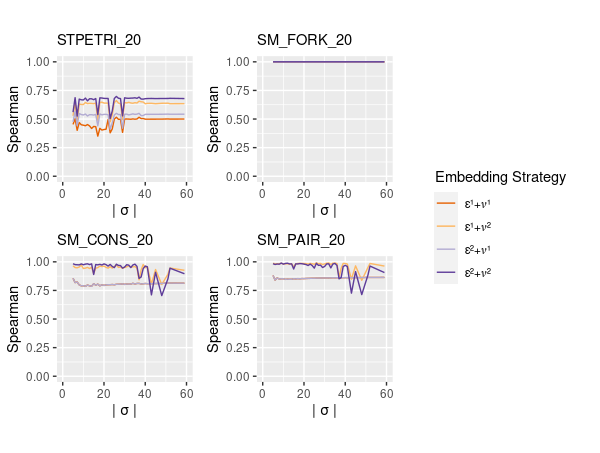
\includegraphics[width=\textwidth]{images/Precision.png}
		\caption{Approximation comparison.}\label{fig:app}
	\end{minipage}\hfill \begin{minipage}{.45\textwidth}
		
		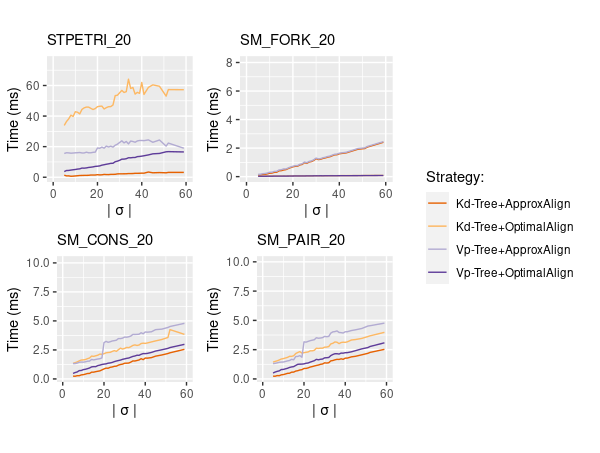
\includegraphics[width=\textwidth]{images/kronos.png}
		\caption{$k$NN alignment benchmark.}\label{fig:kronos}
	\end{minipage}
	\vspace{-0.2cm}
\end{figure*}
\begin{table}[!t]
	\caption{Distinct SWNs and associated sets of \unravelled\ traces discovered from the Sepsis Cases event log.}\label{tab:dataset}
	\centering
	\begin{adjustbox}{width=.49\textwidth}
		\begin{tabular}{crl||cl|c}
			\toprule
			\textbf{Experiment Conf.} $(\mathcal{U})$ & \textit{Model} & $+$\textit{W. Estimator} & $\pmin$& $\;\;|\WCal{\pmin}{n}(P_{\mathcal{U}})|$ \\
			\midrule
			
			\textbf{SM\_CONS\_20} &SplitMiner 2.0  \cite{AugustoCDRP19}       & +\texttt{Constant} &  $\;\;0$ & $157$  \\
			
			\textbf{SM\_FORK\_20} & SplitMiner 2.0  \cite{AugustoCDRP19}      & +Fork \cite{spdwe} &  $\;\;0$ & $32$  \\
			
			
			\textbf{SM\_PAIR\_20} & SplitMiner 2.0  \cite{AugustoCDRP19}      & +PairScale \cite{spdwe} &  $\;\;0$ & $157$ \\
			
			\textbf{STPETRI\_20} & \multicolumn{2}{c||}{Rogge-Solti \cite{RoggeSoltiAW13}} &  $10^{-5}$ & $1612$ \\
			\bottomrule
		\end{tabular}
	\end{adjustbox}
\end{table}


\noindent
\textbf{Properties.}\label{subsub:prop}
We can prove that when two traces $\logtrace$ and ${\nonlogtrace}$ are equivalent (i.e., have the same sequence of labels and the same probability), the kernel computation reduces to $\omega\omega'$. When both weights are $1$, the kernel returns $1$. We call this condition \textit{weak equality} because we cannot possibly prove that when the kernel is equal to $\omega\omega'$ then the two traces we are comparing are equivalent (there could be equal embeddings coming from non-equivalent traces). As shown in Sect. \ref{ex:wheredotiszero}, traces having neither $2$-grams nor transition labels in common have kernel $0$ and vice versa (\textit{strong dissimilarity}). Since weak equality and strong similarity hold, the embedding performs \textit{weakly-ideally}.

%\begin{figure}[!t]
%	\vspace*{-0.5cm}
%	\centering
%	\includegraphics[scale=0.7]{images/counterexample.pdf}
%	\caption{Two TGs, $Q$ (left) and $R$ (right), having a different set of traces but the same embedding representation.}\label{fig:counterexample}
%\end{figure}
%\begin{example}
%	If we use $\epsilon$ (or $\epsilon^2$) and $\nu$ (or $\nu^2$) for $\gorgembed$, we might have a false positive for ``weak equality'' if $Q=(s,s,L,R,w)$ and $R=(s',s',L,R,w)$ are both cycle graphs with $s\neq s'$, $\textit{label}(s)\neq\textit{label}(s')$, $\textit{label}(s)\neq\tau$, and $\textit{label}(s')\neq\tau$. An intuitive example of such situation is presented in Figure \ref{fig:counterexample}: both graphs will have the same frequency for both subtraces and nodes, and therefore have the same  $\epsilon$ and $\nu$ by construction. By having different initial and accepting node with  different labels, we have $\mathcal{W}_0^{\aleph_0}(Q)=\Set{\textup{a(bca)}^n|n\in\mathbb{N}}$ and $\mathcal{W}_0^{\aleph_0}(R)=\Set{\textup{c(abc)}^n|n\in\mathbb{N}}$, thus implying $\mathcal{W}_0^{\aleph_0}(Q)\neq\mathcal{W}_0^{\aleph_0}(R)$ but $k_{\gorgembed}(Q,R)=1$ for $t_f=1$.
%\end{example}
%
%
%\begin{lemma}[Weak Equality]
%	Given two TGs $P=(s,t,L,R,w)$ and $P'=(s',t',L',R',w')$ providing the same set of weighted traces, then $k_{\gorgembed}(P,P')=ww'$ for $t_f=1$.
%\end{lemma}
%%\begin{proof}
%%	\xout{Given Proposition \ref{lem:rewritinglemma} and the positive definition of $\epsilon$ and $\nu$,  we have that $\norm{\hat{\epsilon}-\hat{\epsilon}'}{2}\to 0$ as well as $\norm{\hat{\nu}-\hat{\nu}'}{2}\to 0$, for which we can immediately close the goal.}
%%\end{proof}
%
%%\xout{As per previous observations, we know that}
%Two TGs should have the maximum dissimilarity when all the non $\tau$-nodes have different labels, thus making it impossible to find an alignment, thus implying that they share an utterly dissimilar set of weighted traces:
%
%\begin{lemma}[Strong Dissimilarity]
%	Given two TGs $P=(s,t,L,R,w)$ and $P'=(s',t',L',R',w')$, $k_{\gorgembed}(P,P')=0$ iff. $P$ and $P'$ have a different set of labels with $t_f,w,w'>0$.
%\end{lemma}
%%\begin{proof}
%%	\xout{If we exclude the trivial conditions $t_f=0$, $w=0$ or $w'=0$, the only condition when the kernel returns zero is when  $\Braket{\hat{\epsilon},\hat{\epsilon}'}=0$ and $\Braket{\hat{\nu},\hat{\nu}'}=0$. This implies that, when a component of $\epsilon$ (or $\nu$) is non-zero, the same component of $\epsilon'$ (or $\nu'$) is zero and viceversa. This directly requires that there is a different set of labels associated to the nodes. }
%%\end{proof}
%
%As a corollary of the two lemmas, we have that the proposed embedding performs weakly-ideally as defined in \S\ref{subsec:katk}, as equality condition holds in a relaxed form.
%
%Last, under the assumption that a TG is approximately characterized by $\epsilon$ and $\nu$, we might expect that the TG similarity is characterized by the sum of the distance of both embeddings. Therefore, we show that an increase in both distance embeddings approximately corresponds to a decrease in the kernel output and vice-versa.
%
%\begin{lemma}\label{lem:approxRank}
%	Given two TGs $P=(s,t,L,R,w)$ and $P'=(s',t',L',R',w')$ having respectively the embeddings $(\epsilon,\nu)$ and $(\epsilon',\nu')$, we have that the kernel $k_{\trembed}$ induces an inverse ranking of $\norm{\hat{\epsilon}-\hat{\epsilon}'}{2}+\norm{\hat{\nu}-\hat{\nu}'}{2}$:
%	$$k_{\trembed}(P,P')\appropto 2-(\norm{\hat{\epsilon}-\hat{\epsilon}'}{2}+\norm{\hat{\nu}-\hat{\nu}'}{2})$$
%\end{lemma}
%%\begin{proof}
%%	\xout{Let us use $T=t_f^{|R>0|+|R'>0|}$, $\omega=ww'$, $V=\norm{\hat{\nu}-\hat{\nu}'}{2}$, and $E=\norm{\hat{\epsilon}-\hat{\epsilon}'}{2}$ as shorthands. The goal can be rewritten as $k_{\trembed}(P,P')\appropto 2-(E+V)$. Given that the embeddings $(\epsilon,\nu)$ and $(\epsilon',\nu')$ are normalized kernel function $k_{\gorgembed}$ and that they are always positive definite, then we have that $0\leq E +V\leq 2$, so $0\leq 2-(E+V)\leq 2$. Using Proposition \ref{lem:rewritinglemma}, we can write $k_{\gorgembed}(P,P')$ as follows:}
%%	$$\Rcancel{\left(1-\frac{E}{2}\right)\omega T+\left(1-\frac{V}{2}\right)T=T\left(\omega+1-\frac{E\omega+V}{2}\right)}$$
%%	\xout{Given that the embeddings $(\epsilon,\nu)$ and $(\epsilon',\nu')$ are normalized in $k$ and that they are always positive definite,  we also have that $0\leq E\omega +V\leq 2$ where $0\leq \omega\leq 1$. We can also write  $0\leq \omega+1-\frac{E\omega+V}{2}\leq \frac{2}{T}$. For $\omega,T=1$, we have that $k_{\gorgembed}(P,P')=2-\frac{(E+V)}{2}$. Thus, $0<\omega,T<1$ approximates the expected ranking. }
%%\end{proof}
%
%%\ADD{Such lemma is going to be empirically evaluated in our experiment section.}


\endinput

\smallskip
\noindent
\textbf{Approximate-Ranking Trace Embedder.}
%\label{subsec:ate}
Ranking optimality comes at the cost of a brute-force recomputation of $\goldenrank$ for each trace $\logtrace$ to align. Alternatively, we might avoid the brute-force cost by
%Each embedding $\phi$ entails an associated similarity metric $k_\phi$ (\S\ref{subsec:katk}) and an associated
%distance $d_{k_\phi}$ (Equation \ref{eq:dofk}), hence
%we can compute
computing the embeddings for all the \unravelled\ traces
before the top-$k$ search ensuring that they are independent of the trace to align. %, avoiding the brute-force cost.
%As previously observed,
This computational gain comes with a loss in precision, that our embedding proposal tries to mitigate by overcoming some of the current literature shortcomings:
%; the generation of precise embeddings for graph data with loops is
%NP-complete \cite{GartnerFW03}. %and, in its approximated version, is unable to accurately represent data using low-dimensional
%%vectors \cite{Seshadhri5631}.
%Our proposed embedding ($\gorgembed$) is thus weakly-ideal (\S\ref{subsec:katk}).
%%
%$\gorgembed$ is a variant of the embedding $\trembed$ from \cite{LodhiSSCW02}, which addresses some of its shortcomings.
%Indeed, $\trembed$
%\begin{alphalist}
%	\item is not weakly-ideal, so we cannot numerically assess if two embeddings represent equivalent traces
%	(Example \ref{ex:wheredotiszero});
%	\item does not characterize $\tau$-moves, so the probabilities of the initial and final $\tau$-moves are not preserved; and
%	\item is affected by numerical errors from finite arithmetics: longer traces $\nonlogtrace$ generated from skewed probability
%	distributions $G.\Lambda^i$ yield greater truncation errors, as smaller $\lambda^i$ components for bigger
%	$i<|\nonlogtrace|$ are ignored, preventing a complete numerical vector characterization of  $\nonlogtrace$ in practice.
%\end{alphalist}
%%
%To overcome these shortcomings we
	 propose a weakly-ideal embedding
 preserving probabilities from and to $\tau$ transitions, and
 mitigating the numerical truncation errors induced by trace length and probability distribution skewness through two
sub-embedding strategies, $\epsilon$ for transition correlations in $\tasks^2$ and $\nu$ for transition label frequency in $\tasks$\cite{Bergami21}.
%

In order to meet the goal, we need to first transform an SWN into a TG: first, for each model trace $\nonlogtrace$ we need to restrict the TG into a \textit{weighted} TG $G_\nonlogtrace=(TG_{\nonlogtrace},\omega_\nonlogtrace)$, where $TG_{\nonlogtrace}$ contains only the nodes generating $\nonlogtrace$, thus restricting the associated matrices $L$ (and $R$) into $L_\nonlogtrace$ (and $R_\nonlogtrace$). $\omega_\nonlogtrace$ is then exploited to preserving probabilities from initial (and to final) $\tau$ transitions. Such $\omega$ can be computed as $\omega := 1-\prod_{\Ind{0}\cdots\Ind{n}\in\seqs{\sigma'}{ \closed{G}}}\Big(1-(\textit{ifte}(\mathbf{1}_{L_{\sigma'}(\Ind{0})=\tau},[R_{\sigma'}]_{\Ind{0}\Ind{1}})\textit{ifte}(\mathbf{1}_{L_{\sigma'}(\Ind{n})=\tau},[R_{\sigma'}]_{\Ind{n-1}\Ind{n}})\Big)$
where $\textit{ifte}(x,y):=x(y-1)+1$ returns $y$ if $x=1$ and $1$ otherwise. %We denote the set of all the $\closed{G}_\nonlogtrace$ as $\TBf{\pmin}{4}(\closed{G})$.
%The graph weight $\omega$ derives from the outgoing edges of the initial node and the ingoing edges of the accepting node;
%such nodes are labeled as $\tau$. %Since the embedding strategy from \cite{LodhiSSCW02} considers only visible
%transitions, and the trace extraction process discards the $\tau$ information, we use $\omega$ to preserve such information.
%We call the pair consisting of a transition graph and a graph weight a \emph{weighted transition graph}.
%\begin{example}\label{ex:neue}
%\end{aligned}$$
\tablename~\ref{tab:proj} shows the projected transition graphs associated to  traces from Example \ref{ex:rankingTaus}, where  all the $\tau$-labeled nodes are removed as required.
%\end{example}
%	
%
%
%Since a trace embedding for $\nonlogtrace$ representing the transitions in $\closed{\tg}.\Lambda$ requires an intermediate
%TG representation, each $\nonlogtrace$ is mapped to a weighted TG $(\tg_\nonlogtrace,\omega)$:
%%
%\begin{definition}[trace projection]
%	Let $\closed{G}=(V,s,t,L,R)$ be a $\tau$-closed TG, and $\pmin\in(0,1]$. The $\closed{G}$ \emph{projection} over the trace
%	$\nonlogtrace$ is the weighted TG $(\closed{G}_\nonlogtrace,\omega)$, where $\closed{G}_\nonlogtrace$ is the TG
%	$(V_\nonlogtrace,s,t,L_\nonlogtrace,R_\nonlogtrace)$ where
%	$V_\nonlogtrace$ contains the nodes generating $\nonlogtrace$ from $\closed{G}$	
%	(i.e., $\seqs{\sigma'}{ \closed{G}}$) and
%	$L_\nonlogtrace$ and $R_\nonlogtrace$ are the restrictions of $L$ and $R$ to $V_\nonlogtrace$; and
%	$\omega := 1-\prod_{\Ind{0}\cdots\Ind{n}\in\seqs{\sigma'}{ \closed{G}}}\Big(1-(\textit{ifte}(\mathbf{1}_{L_{\sigma'}(\Ind{0})=\tau},[R_{\sigma'}]_{\Ind{0}\Ind{1}})\textit{ifte}(\mathbf{1}_{L_{\sigma'}(\Ind{n})=\tau},[R_{\sigma'}]_{\Ind{n-1}\Ind{n}})\Big)$
%	where $\textit{ifte}(x,y):=x(y-1)+1$ returns $y$ if $x=1$ and $1$ otherwise. We denote the set of all the $\closed{G}_\nonlogtrace$ as $\TBf{\pmin}{4}(\closed{G})$.%\todo{need to understand this}
%	%\dots
%	%		
%	%		\dots we generate a set $\TBf{\pmin}{n}(\closed{G})$ of projected TGs $P$ for each trace in $\WCal{\pmin}{n}(P)$ as follows: for each weighted trace $\braket{\nonlogtrace,\probskip{\nonlogtrace}}\in\WCal{\pmin}{n}(P)$ generated from a path $\pi_\nonlogtrace=s\to n_2\rightsquigarrow n_m\to t$ over $R$, we generate a TG $P_\nonlogtrace=(s',t',L_\nonlogtrace,R_\nonlogtrace,\omega')$, where \begin{inparaenum}[\it (i)]
%	%			\item $s'=s$ if $\textit{label}(s)\neq \tau$ and $t'=n_2$ otherwise,
%	%			\item $t'=t$ if $\textit{label}(t)\neq \tau$ and $t'=n_m$ otherwise,
%	%			\item $L_\nonlogtrace$ (and $R_\nonlogtrace$) is the submatrix of $L$ (and $R$) over the non-$\tau$ labeled notes in $\pi_\nonlogtrace$ and the labels from $\nonlogtrace$,
%	%			\item $\omega'$ is initialized by $\omega$ and then multiplied by $[R]_{s,n_2}$ (and also $[R]_{n_m,t}$) if $\textit{label}(s)=\tau$ (and  $\textit{label}(t)=\tau$).
%	%		\end{inparaenum}
%\end{definition}
%	
%\begin{table}[!t]
%	\caption{Projections of $\tg$ over $\net$-traces of length $4$.}\label{tab:proj}
%	\centering
%	\resizebox{.3\textwidth}{!}{\begin{tabular}{>{\centering\arraybackslash} m{1cm}| >{\centering\arraybackslash} m{4cm} >{\centering\arraybackslash} m{1cm} >{\centering\arraybackslash} m{1cm} }
%			\toprule
%			$\nonlogtrace$&$G_\nonlogtrace$&$l$&$\omega$\\
%			\midrule
%			$\const{a}$ & \includegraphics{images/trace_a} & $1$ & $\color{violet}\pa\pf$\\
%			$\const{cb}$ & \includegraphics{images/trace_cb} & $2$ & $\color{violet}\pb$\\
%			$\const{aaa}$ & \includegraphics{images/trace_a_loop} & $3$ & $\color{violet}\pa\pf$\\
%			$\const{caa}$ & \includegraphics{images/trace_caa} & $3$ & $\color{violet}\pb\pf$\\
%			%			\bottomrule
%			%	\end{tabular}}\qquad \qquad 	
%			%	\resizebox{.3\textwidth}{!}{\begin{tabular}{>{\centering\arraybackslash} m{1cm}| >{\centering\arraybackslash} m{4cm} >{\centering\arraybackslash} m{1cm} >{\centering\arraybackslash} m{1cm} }
%			%	\toprule
%			%	$\nonlogtrace$&$G_\nonlogtrace$&$l$&$\omega$\\
%			%	\midrule
%			$\const{aa}$ & \includegraphics{images/trace_aa} & $2$ & $\color{violet}\pa\pf$\\
%			$\const{ca}$ & \includegraphics{images/trace_ca} & $2$ & $\color{violet}\pb\pf$\\
%			\begin{tabular}{l}aaaa\end{tabular} & \includegraphics{images/trace_a_loop} & $4$ & $\color{violet}\pa\pf$\\
%			$\const{caaa}$ & \includegraphics{images/trace_ca_loop} & $4$ & $\color{violet}\pb\pf$\\
%			\bottomrule
%	\end{tabular}}
%	%\vspace{-0.2cm}
%\end{table}
\begin{table}[!t]
	\caption{Projections over $\net$-traces of length $4$.}\label{tab:proj}
	\centering
	\resizebox{.3\textwidth}{!}{\begin{tabular}{>{\centering\arraybackslash} m{1cm}| >{\centering\arraybackslash} m{4cm} >{\centering\arraybackslash} m{1cm} >{\centering\arraybackslash} m{1cm} }
			\toprule
			$\nonlogtrace$&$G_\nonlogtrace$&$l$&$\omega_\nonlogtrace$\\
			\midrule
			$\const{a}$ & \includegraphics{images/trace_a} & $1$ & $\color{violet}\pa\pf$\\
			$\const{cb}$ & \includegraphics{images/trace_cb} & $2$ & $\color{violet}\pb$\\
			$\const{aaa}$ & \includegraphics{images/trace_a_loop} & $3$ & $\color{violet}\pa\pf$\\
			$\const{caa}$ & \includegraphics{images/trace_caa} & $3$ & $\color{violet}\pb\pf$\\
			$\const{aa}$ & \includegraphics{images/trace_aa} & $2$ & $\color{violet}\pa\pf$\\
			$\const{ca}$ & \includegraphics{images/trace_ca} & $2$ & $\color{violet}\pb\pf$\\
			\begin{tabular}{l}aaaa\end{tabular} & \includegraphics{images/trace_a_loop} & $4$ & $\color{violet}\pa\pf$\\
			$\const{caaa}$ & \includegraphics{images/trace_ca_loop} & $4$ & $\color{violet}\pb\pf$\\
			\bottomrule
	\end{tabular}}
	\vspace{-0.2cm}
\end{table}
Our proposed embedding $\gorgembed$ \cite{Bergami21} can be now exploited for each $G_\nonlogtrace$ as follows:
%Our proposed embedding $\gorgembed$ is computed for each $wTG_\nonlogtrace$. The goal is to use
%$k_{\gorgembed}$ for ranking all the traces generated by \unravelling\ via such graphs. We extend $\trembed$ %from
%%\cite{LodhiSSCW02} including the associated probabilities, and
%by making the ranking induced by $k_{\gorgembed}$ the inverse of
%that induced by the
%sum of the following distances: the transition correlations $\epsilon$ and the transition label frequency $\nu$.
%We need that the desired properties of $\gorgembed$ are independent of the characterization of $\epsilon$ over the
%$2$-grams in $\tasks^2$ and $\nu$ over the labels in $\tasks$. %which  provide different embedding strategies. Therefore, our
%%$\gorgembed$ embedding is defined for any weighted TG.


%\begin{table}[!t]
%	\centering
%	\caption{Embedding representation for the TG $P$ in \figurename~\ref{fig:closed} and the trace $\logtrace=\textup{caba}$ after representing it as in \figurename~\ref{fig:sigmastar}. Please note that we restrict $\trace_\tau^2$ to the one from $P$.}\label{tab:emb1}
%		\begin{tabular}{l|l|l|l|l|l|l|}
%	\toprule
%	& a    & b                                                   & c    & aa   & ca   & cb   \\
%	\midrule
%	$\gorgembed(P)$ & $9.94\cdot10^{-25}$ & $1.18\cdot 10^{-26}$ & $1.04\cdot10^{-25}$ & $4.45\cdot 10^{-25}$ & $6.22\cdot10^{-25}$ & $8.29\cdot10^{-26}$\\
%	$\gorgembed(P_{\logtrace})$ & $8.16\cdot10^{-17}$ & $4.08\cdot 10^{-17}$ & $4.08\cdot10^{-17}$ & $4.37\cdot 10^{-17}$ & $1.03\cdot10^{-16}$ & $4.37\cdot10^{-17}$\\
%	\bottomrule
%\end{tabular}
%\end{table}
\begin{definition}[G-Embedding]\label{def:ppne}
	%Given a finite set of non-empty labels $\trace_\tau =\trace\backslash\{\tau\}$, $\trace_\tau^2$ denotes all the possible pair of labels associated to paths ${\color{green}\alpha}\rightsquigarrow{\color{green}\beta}$ and $\trace_\tau$ denotes the set of all the possible non-$\tau$ node labels. Therefore, it is always possible to enumerate $\trace_\tau^2\cup\trace_\tau$ via an enumeration by a bijection $\iota\colon \trace_\tau^2\cup\trace_\tau\to  N$, where $N\subset \mathbb{N}_{\neq 0}$ and $\max N=|N|$.
	Given a weighted TG $G_\nonlogtrace=(TG_{\nonlogtrace},\omega_\nonlogtrace)$ and a tuning parameter $t_f\in[0,1]$, the \emph{TG-Embedding} is
	$$\gorgembed_{i}(G_\nonlogtrace):=\begin{cases}
	\omega_\nonlogtrace \frac{\epsilon_\const{ab}(TG_{\nonlogtrace})}{\|\epsilon\|_2}\;t_f^{|R>0|}\, & {i}=\const{ab}\in\tasks^2\\
	\frac{\nu_\const{a}(TG_{\nonlogtrace})}{\|\nu\|_2}\;\;\;\,t_f^{|R>0|}\, & {i}=\const{a}\in\tasks\\
	\end{cases}$$
	where $\nu$ and $\epsilon$ represent the embeddings associated to $L$ and $L,R$: $\epsilon$  returns
	$\epsilon_\const{ab}=0$ for the $2$-grams $\const{ab}$ not represented by the TG, and either $\nu$ always returns the empty
	vector or $\nu_\const{a}(G)=0$ iff the labels $\const{a}\in\tasks$ that are associated to no vertex in $V$.
\end{definition}
%
Here, ${\max\arg}_{\nonlogtrace\in \WCal{\pmin}{n}, G_\nonlogtrace\in\TBf{p}{n}(P)} k_{\gorgembed}(G_\logtrace, G_{\nonlogtrace})$ returns the best approximated trace alignment for a log trace represented as $G_{\logtrace}$. %\xout{Similarly, we can provide the TG $P\in\mathbf{P}$ providing the best approximated alignment for $P_{\logtrace}$ as $\underset{P}{\max\arg}\underset{ P_\trace\in\mathbf{P}_p^n(P)}{\max} k_{\gorgembed}(P_\trace, P_{\logtrace})$.}¯
%
\begin{table}[!t]
	\caption{Different sub-embeddings ($\epsilon^1$, $\epsilon^2$, $\nu^1$, and $\nu^2$) for $\gorgembed$.}\label{tab:embedstrat}
	\centering
	\resizebox{.49\textwidth}{!}
	{\begin{tabular}{c|c|c}
			\toprule
			& $x=1$ & $x=2$ \\
			\midrule
			$\epsilon^x_\const{ab}(G):=$ & $\label{eq:epsilon}
			\sum_{i=1}^l{\lambda^i}\frac{[LR^iL^t]_\const{ab}}{\sum_{\const{a'b'}\in\tasks^2}R^i_\const{a'b'}}$ & $
			\sum_{i=1}^l\lambda^i[\Lambda^i]_\const{ab}$\\
			$\nu^x_\const{a}(G):=$ & $\frac{1}{c}\sum_{\nonlogtrace'\in \ptraces{G}{0}}\frac{|\Set{\nonlogtrace_i'\in\nonlogtrace'|\const{a}\in\tasks\wedge \nonlogtrace'_i=\const{a}}|}{|\nonlogtrace'|}$ & $0$ \\
			\bottomrule
	\end{tabular}}
\end{table}
%
We choose two possible interchangeable definitions for $\nu$ and $\epsilon$ shown in \tablename~\ref{tab:embedstrat}, where $l$
is the path length, and $c$ for $\nu^1$ is a normalization factor such that $\sum_{\const{a}\in\tasks}\nu^1_\const{a}(P)=1$;
$\nu^2$ completely ignores the label frequency contribution; $\epsilon^2$ is the embedding $\trembed$ from Sect. \ref{subsec:katk};
and $\epsilon^1$ and $\epsilon^2$ only differ from the normalization. $t_f\in [0,1]$ and $\lambda\in (0,1]$ are tuning
parameters that can be inferred from the available data. %\cite{DriessensRG06}.
The latter describes the decay factor, while $t_f$
represents the relevance of our embedding representation as the number of edges within $\closed{G}_\nonlogtrace$ increases.
We choose $t_f=0.0001$ and $\lambda=0.07$.
%
This representation is independent of the representation of the trace to be aligned and does not have to be
recomputed for each alignment.



%When the transition matrix is ergodic \cite{StocasticCC},  the transition matrix embedding converges to $\epsilon(R)_{\color{green}\alpha\beta}=[(\mathbf{I}-\lambda\Lambda)^{-1}]_{\color{green}\alpha\beta}$ \cite{GartnerFW03} for $n\to+\infty$.

%\begin{table*}[!t]
%	\centering
%	\caption{Embeddings for $\net$-traces of maximum length $4$ and $\logtrace=\const{caba}$.}\label{tab:emb2}\label{tab:embsitar}
%	\resizebox{\textwidth}{!}{\begin{tabular}{lllllllllllll}
%			\toprule
%			& $\const{a}$    & $\const{b}$                                                   & $\const{c}$    & $\const{aa}$  & $\const{ab}$   & %$\const{ac}$   & $\const{ba}$  & $\const{bb}$   & $\const{bc}$   & $\const{ca}$   & $\const{cb}$  & $\const{cc}$  \\
%			\midrule		
%			$\gorgembed(TG_\const{aaaa})$ & $1.00\cdot 10^{-24}$ & $0$   & $0$   & $6.44\cdot 10^{-26}$ & $0$& $0$& $0$& $0$& $0$    &$0$& $0$& $0$ \\
%			$\gorgembed(\overline{G}_\const{aaa})$  & $1.00\cdot 10^{-24}$ & $0$   & $0$   & $1.29\cdot 10^{-25}$ & $0$& $0$& $0$& $0$& $0$    &$0$& $0$& $0$ \\
%			$\gorgembed(\overline{G}_\const{aa})$   & $1.00\cdot 10^{-24}$ & $0$   & $0$   & $2.57\cdot 10^{-25}$ & $0$& $0$& $0$& $0$& $0$    &$0$& $0$& $0$ \\
%			$\gorgembed(\overline{G}_\const{a})$    & $1.00\cdot 10^{-4}$  & $0$   & $0$   & $0$   & $0$& $0$& $0$& $0$& $0$    &$0$& $0$& $0$ \\
%			$\gorgembed(\overline{G}_\const{caa})$  & $7.07\cdot 10^{-25}$ & $0$   & $7.07\cdot 10^{-25}$ & $1.46\cdot 10^{-25}$ & $0$& $0$& $0$& $0$& $0$    &$2.05\cdot 10^{-25}$& $0$& $0$ \\
%			$\gorgembed(\overline{G}_\const{ca})$   & $7.07\cdot 10^{-25}$ & $0$   & $7.07\cdot 10^{-25}$ & $0$   & $0$& $0$& $0$& $0$& $0$    &$1.00\cdot 10^{-8}$& $0$& $0$ \\
%			$\gorgembed(\overline{G}_\const{cb})$   & $0$   & $7.07\cdot 10^{-25}$ & $7.07\cdot 10^{-25}$ & $0$   & $0$& $0$& $0$& $0$& $0$    &$0$ & $4.29\cdot 10^{-9}$& $0$ \\
%			$\gorgembed(\overline{G}_\const{caaa})$ & $7.07\cdot 10^{-25}$ & $0$   & $7.07\cdot 10^{-25}$ & $1.03\cdot 10^{-25}$ & $0$& $0$& $0$& $0$& $0$    &$7.20\cdot 10^{-26}$ & $0$& $0$ \\
%			\bottomrule
%			$\gorgembed(\overline{G}_\const{caba})$ & $8.16\cdot10^{-17}$ & $4.08\cdot 10^{-17}$ & $4.08\cdot10^{-17}$ & $4.37\cdot 10^{-17}$ &  $0$& $0$& $0$ & $0$ & $0$    & $1.03\cdot10^{-16}$ & $4.37\cdot10^{-17}$& $0$ \\
	%		\bottomrule
	
%\end{tabular}}
	
%\end{table*}
\begin{example}
	%\small \label{ex:withpaths} %After generating all the TGs for the \unravelled\ traces (Example \ref{ex:neue}), we further associate a sub-embedding $\epsilon$ using the $2$-grams included in the model traces.\footnoteref{fn:caveat}
	%Given $\nonlogtrace_\tau=\Set{a,b,c}$, the embedding space is of size $6$: three features (computed using $\nu$) correspond to the labels of the non-$\tau$ vertices in $\nonlogtrace_\tau$, i.e., $\{a,b,c\}$, and other three features (computed using $\epsilon$) correspond to the $2$-grams subsequences that are also traces in $W^4_0(P)$, i.e., $\{aa,ca,cb\}$. Therefore, $\{a,b,c,aa,ca,cb\}\subset \nonlogtrace_\tau^2\cup\nonlogtrace_\tau$ is the whole set of features describing both the label and the transition matrix, so $\gorgembed$ is a vector with 6 dimensions.
	%\xout{The embedding associated to $P$ is described in \tablename~\ref{tab:emb1} as $\gorgembed(P)$: it shows that doing ${\color{green}a}\rightsquigarrow{\color{green}a}$ is more probable than doing  ${\color{green}c}\rightsquigarrow{\color{green}a}$. Also, given that both the probability of performing ${\color{green}c}\overset{1}{\rightsquigarrow}{\color{green}b}$ is relatively low and trace $\color{green}cb$ is relatively infrequent, ${\color{green}c}{\rightsquigarrow}{\color{green}b}$ is less probable than any other subtrace. If we now consider the single nodes, $\color{green}c$ shares a subset of traces with $\color{green}a$ where $\color{green}a$ is more frequent than $\color{green}c$, and therefore the score of the former is higher than the one of the latter. Also, the score associated to the single node $\color{green}b$ is lower than the one for the single node $\color{green}c$ because $\color{green}b$ is less frequent and appears in less probable traces than $\color{green}c$: in particular, $\color{green}c$ appears in \textit{ca}, which is more probable than \textit{cb}.}
	\tablename~\ref{tab:emb2} shows the embeddings $\gorgembed(\overline{G}_\nonlogtrace)$ generated from \tablename~\ref{tab:proj}, where the $l=|\nonlogtrace|$ for each \unravelled trace.
	After representing trace $\logtrace=\const{caba}$ as a sequence graph, we find its
	embedding $\gorgembed(\overline{G}_{\logtrace})$ with strategies $\epsilon^1$ and $\nu^1$
	{as} in \tablename~\ref{tab:embsitar}: $\const{a}$ is the most frequent label and $\const{b}$ and $\const{c}$ are equiprobable.
	The $2$-gram $\const{ca}$ appears twice in the trace set and is more frequent than other $2$-grams.
\end{example}
%
These sub-embeddings satisfy the conditions required by the G-Embedding.
\begin{lemma}
	\label{lem:addedForOurPropos}
	The sub-embeddings in Table~\ref{tab:embedstrat} satisfy the requirements from Definition~\ref{def:ppne}.
\end{lemma}


The kernel $k_{\gorgembed}$ associated to $\gorgembed$ is {a function of the distance  $\|\hat{\epsilon}(G)-\hat{\epsilon}(G')\|_2^2$ and $\|\hat{\nu}(G)-\hat{\nu}(G')\|_2^2$ for traces $\logtrace$ and ${\nonlogtrace}$.}
%

\begin{proposition}
	\label{lem:rewritinglemma}
	Given {two weighted TGs} $(G,\omega)$ and $(G',\omega')$ with $G=(s,t,L,R)$ and $G'=(s',t',L',R')$, the definition of
	$k_\gorgembed$ is expanded to
	$\begin{aligned}
	%k_{\gorgembed}(G,G')=&
	 \omega\omega't_f^{|R>0|+|R'>0|}\left(1-\frac{\norm{\hat{\epsilon}(G)-\hat{\epsilon}(G')}{2}^2}{2}\right)+\\t_f^{|R>0|+|R'>0|}\left(1-\frac{\norm{\hat{\nu}(G)-\hat{\nu}(G')}{2}^2}{2}\right)
	\end{aligned}$
\end{proposition}

When $\hat{\epsilon}(G)$ and $\hat{\epsilon}(G')$ are affected by truncation errors
(i.e., $\norm{\hat{\epsilon}(G)-\hat{\epsilon}(G')}{2}^2\to 0$), the $\nu$ strategy intervenes as a backup ranking. The first
term of the sum does not affect the ranking, as it reduces to a constant factor.

%\xout{Given that we can now follow Definition \ref{def:ppne} for representing a trace $\trace$ as a proper embedding after transforming it as a TG $P_{\logtrace}$ (\S\ref{subsec:katk}), we can find the TG $P$ providing the best approximate match with  a trace $\trace$ as follows:}
%\[\Rcancel{\underset{{P}}{\max\arg}\;k_{\gorgembed}(P,T)}\]
%\xout{Still, this TG matching strategy does not allow to find the trace maximizing such score.} %To assess such problem, the next section is going to determine both an exact (\S\ref{subsec:exbkptap}) and an approximated strategy (\S\ref{subsec:akptap}) for probabilistically matching one single trace from the TG.
%
%\xout{Given the characterization of a TG as in \S\ref{subsec:ppn} and the embedding strategy proposed in Definition \ref{def:ppne}, We can \ADD{now} generate an embedding for each possible weighted trace $\braket{\trace,\probskip{\trace}}\in\mathcal{W}_p^n(P)$ for a given TG $P$ as described in the following definition:}



\begin{table}[!t]
	\caption{Distinct SWNs and associated sets of \unravelled\ traces discovered from the Sepsis Cases event log.}\label{tab:dataset}
	\centering
	\begin{adjustbox}{width=.49\textwidth}
		\begin{tabular}{crl||cl|c}
			\toprule
			\textbf{Experiment Conf.} $(\mathcal{U})$ & \textit{Model} & $+$\textit{W. Estimator} & $\pmin$& $\;\;|\WCal{\pmin}{n}(P_{\mathcal{U}})|$ \\
			\midrule
			
			\textbf{SM\_CONS\_20} &SplitMiner 2.0  \cite{AugustoCDRP19}       & +\texttt{Constant} &  $\;\;0$ & $157$  \\
			
			\textbf{SM\_FORK\_20} & SplitMiner 2.0  \cite{AugustoCDRP19}      & +Fork \cite{spdwe} &  $\;\;0$ & $32$  \\
			
			
			\textbf{SM\_PAIR\_20} & SplitMiner 2.0  \cite{AugustoCDRP19}      & +PairScale \cite{spdwe} &  $\;\;0$ & $157$ \\
			
			\textbf{STPETRI\_20} & \multicolumn{2}{c||}{Rogge-Solti \cite{RoggeSoltiAW13}} &  $10^{-5}$ & $1612$ \\
			\bottomrule
		\end{tabular}
	\end{adjustbox}
\end{table}



\begin{example}%\small \label{ex:11}
	The products $k_{\gorgembed}(\logtrace,\nonlogtrace)=\braket{\gorgembed(\overline{G}_\logtrace),\;\gorgembed(\overline{G}_{\nonlogtrace})}$
	with sub-embedding $\nu^1$ and $\epsilon^1$, for each trace $\nonlogtrace$ appear in
	\tablename~\ref{tab:rank3} along optimal-ranking $\goldenrank$. $k_{\gorgembed}$ approximates the optimal-ranking as it tends to rank the transition graphs $\closed{G}_\nonlogtrace$ (generated from $\overline{G}$ via projection) similarly to the traces over $\mathcal{R}$.
\end{example}
%
%\begin{example}\label{ex:moreskew}
%	\xout{Let us suppose to change the probability distribution associated with the $P$'s edges, so that it becomes more skewed and that some traces are relatively more probable than others. Let us set $p_1=p_2=0.5$, $p_3=0.9$, $p_6=0.1$, $p_4=0.3$, and $p_5=0.7$, so that the initial choice is equiprobable but performing a loop is more probable than terminating the path. We keep the other tuning parameters as in Example \ref{ex:withpaths}. In this case, we generate the following set of weighted traces:}
%	$$\begin{aligned}
%	\Rcancel{\mathcal{W}_0^4(P)=\{}&\Rcancel{\braket{cb,0.35},\braket{a,0.05},\braket{aa,0.045},\braket{aaa,0.0405},}\\
%	&\Rcancel{\braket{aaaa,0.03645},\braket{ca,0.015},\braket{caa,0.0135},\braket{caaa,0.01215}\}}\\
%	\end{aligned}$$
%	\xout{Let us also assume that we want to align these traces in a probabilistic way with the query $\logtrace=\textup{caba}$: the distance ($d$) and similarity ($s_d$) scores will be still the same, while the associated probabilities will vary. The expected ranking by multiplying weight with similarity is represented in \tablename~\ref{tab:witherror}.}
%	
%	%\xout{As a consequence of the different probability distribution associated to the edges, a different set of embedding will be generated for each trace of interest while the TG $T$ associated to $\logtrace$ will be kept the same. \tablename~\ref{tab:witherror} represents the ranking induced by the kernel $k_{\gorgembed}$ over this different set of vectors by ranking the traces in descendant order of $k_{\gorgembed}$. As we might notice, the more skewed edge probability distribution introduced more errors in the ranking result: while the largest ranking subsequence (marked in blue) always starts from the best-expected trace \textit{cb}, this element now appears in the third position, and the position of traces \textit{caa} and \textit{aaaa} is swapped.}
%	
%\end{example}
%\begin{table}[!t]
%	\centering
%	\caption{Expected ranking of the paths from Example \ref{ex:moreskew} with the trace $\logtrace=\textup{caba}$. The cost function is the one from \cite{LeoniM17} and its normalized similarity score has $c=5$. Traces are ranked by decreasing kernel $k_{\gorgembed}$ value: slight changes in the expected expected order are circled, the others are marked in red.}\label{tab:witherror}
%	\begin{tabular}{lc|ll|cc|l}
%		\toprule
%		
%		\multirow{2}{*}{$\trace$} &
%		\multirow{2}{*}{$d(\trace,\logtrace)$} &
%		\multicolumn{2}{c|}{$\mu_{\logtrace}$} &
%		\multirow{2}{*}{$\approx s_d(\trace,\logtrace)\cdot \probskip{\trace}$} &
%		\multirow{2}{*}{$k_{\gorgembed}(\trace,\logtrace)$}&
%		\multirow{2}{*}{\textit{expected ranking}}\\
%		
%		\cline{3-4} &&  $\langle \probskip{\trace}$ &  $,\,s_d(\trace,\logtrace)\rangle $ && \\
%		
%		\midrule
%		{a}  & $3$ & $0.05$ & $\;\; 0.6250$  & $0.03125$ & $8.16497\cdot 10^{-16}$ & \textbf{\color{red}3}\\
%		{ca}  & $2$ & $0.015$ & $\;\; 0.7142$ & $0.01071$ & $1.30623\cdot 10^{-18}$ & \textbf{\color{red}7}\\
%		{cb}  & $2$ & $0.35$ & $\;\; 0.7142$ & $0.25000$ & $1.01399\cdot10^{-18}$ & \textbf{\color{blue}1}\\
%		{aa}  & $2$ & $0.045$ & $\;\; 0.7142$ & $0.03214$ & $1.01894\cdot10^{-30}$ & \textbf{\color{blue}2}\\
%		{aaa}  & $2$ & $0.0405$ & $\;\; 0.7142$ & $0.02893$ & $9.98696\cdot10^{-31}$ & \textbf{\color{blue}4}\\
%		{caa}  & $1$ & $0.0135$ & $\;\; 0.8333$ & $0.01125$ & $9.96052\cdot10^{-31}$ & \textbf{\color{blue}\ding{177}}\\
%		{aaaa}  & $3$ & $0.03645$ & $\;\; 0.7142$ & $0.02603$ & $9.80476\cdot10^{-31}$ & \textbf{\color{blue}\ding{176}}\\
%		{caaa}  & $1$  & $0.01215$ & $\;\; 0.8333$ & $0.01012$ & $9.52398\cdot 10^{-31}$ & \textbf{\color{blue}8}\\
%		\bottomrule
%	\end{tabular}
%\end{table}
%\begin{table}[!t]
%	\caption{Comparison between the ranking induced by the expected ranking $\goldenrank$ and the proposed kernel $k_{\gorgembed}$ with embedding strategies $\epsilon^2$ and $\nu^1$: arrows $\boldsymbol{\downarrow}$ remark the column of choice under which we sort the rows (i.e., ranking).}\label{tab:compLit}
%	\centering
%	\resizebox{.9\textwidth}{!}{\begin{tabular}{l|ll|cc}
%			\toprule
%			
%			{$\trace$} &
%			%\multirow{2}{*}{$d(\trace,\logtrace)$} &
%			%\multicolumn{2}{c|}{$\mu_{\logtrace}$} &
%			$( \probskip{\trace}$ &  $,\,\boldsymbol{\downarrow} s_d(\trace,\logtrace)) $ &
%			{$=\goldenrank(\trace,\logtrace)$} &
%			{$k_{\gorgembed}(P_\trace,P_{\logtrace})$} \\
%			
%			
%			\midrule
%			$\const{caa}$  & $0.035$ & $\;\; 0.8333$ & $0.0292$ & $1.03498\cdot10^{-40}$\\
%			$\const{caaa}$  &  $0.0175$ & $\;\; 0.8333$ & $0.0145$ & $8.94997\cdot10^{-41}$ \\
%			$\const{a}$  & $0.4$ & $\;\; 0.6250$  & $0.2500$ & $8.16497\cdot10^{-21}$\\
%			$\const{aaaa}$ & $0.05$ & $\;\; 0.6250$ & $0.0357$ & $8.20640\cdot10^{-41}$\\
%			$\const{aa}$  & $0.2$ & $\;\; 0.7142$ & $0.1428$ & $9.96007\cdot10^{-41}$ \\
%			$\const{aaa}$  & $0.1$ & $\;\; 0.7142$ & $0.0714$ & $8.41263\cdot10^{-41}$\\
%			$\const{ca}$  &  $0.07$ & $\;\; 0.7142$ & $0.0500$ & $1.45079\cdot10^{-24}$\\
%			$\const{cb}$  &  $0.06$ & $\;\; 0.7142$ & $0.0428$ & $8.52070\cdot10^{-25}$\\
%			\bottomrule
%		\end{tabular}\quad \begin{tabular}{l|c}
%			\toprule
%			
%			{$\trace$} &
%			{$\boldsymbol{\downarrow}\goldenrank(\trace,\logtrace)$} \\
%			
%			
%			\midrule
%			$\const{a}$  &  $0.2500$ \\
%			$\const{aa}$  &  $0.1428$  \\
%			$\const{aaa}$  & $0.0714$ \\
%			$\const{ca}$  &   $0.0500$\\
%			$\const{cb}$  & $0.0428$ \\
%			$\const{aaaa}$  &  $0.0357$ \\
%			$\const{caa}$  &  $0.0292$ \\
%			$\const{caaa}$  &   $0.0145$ \\
%			\bottomrule
%		\end{tabular}\quad	\begin{tabular}{l|c}
%			\toprule
%			
%			{$\trace$} &
%			{$\boldsymbol{\downarrow}k_{\gorgembed}(P_\trace,P_{\logtrace})$} \\
%			
%			
%			\midrule
%			{a}  & $8.16497\cdot10^{-21}$ \\
%			{ca}  &   $1.45079\cdot10^{-24}$\\
%			{cb}  &   $8.52070\cdot10^{-25}$\\
%			{caa}  & $1.03498\cdot10^{-40}$\\
%			{aa}  &  $9.96007\cdot10^{-41}$ \\
%			{caaa}  &  $8.94997\cdot10^{-41}$ \\
%			{aaa}  &  $8.41263\cdot10^{-41}$\\
%			{aaaa}  & $8.20640\cdot10^{-41}$\\
%			\bottomrule
%	\end{tabular}}
%	
%	\centering
%	\begin{tabular}{lc|l}
%		\toprule
%		%\multicolumn{3}{c||}{Example \ref{ex:withpaths}} %&
%		%\multicolumn{3}{c}{Example \ref{ex:moreskew}}\\
%		%\hline
%		$\trace$ &  $k_{\gorgembed}(P_\trace,P_{\logtrace})$ & $\goldenrank(\trace,\logtrace)$\\ %&
%		%$\trace$ &  $k_{\gorgembed}(\trace,\logtrace)$ & \textit{exp. ranking}\\
%		\midrule
%		
%		a & $\;8.16497\cdot10^{-21}$ & \textbf{\color{blue}1} \\%& a & $\;8.16497\cdot 10^{-21}$ & \textbf{\color{red}3} \\
%		ca & $\;1.45079\cdot10^{-24}$ & \textbf{\color{blue}4} \\%& ca &  $\;1.45079\cdot 10^{-24}$ & \textbf{\color{red}7}\\
%		cb & $\;8.52070\cdot10^{-25}$ & \textbf{\color{blue}5} \\%& cb & $\;8.52070\cdot10^{-25}$& \textbf{\color{blue}1}\\
%		caa & $\;1.03498\cdot10^{-40}$ & \textbf{\color{blue}7} \\%& aa & $\;9.29342\cdot10^{-41}$ & \textbf{\color{blue}2}\\
%		aa & $\;9.96007\cdot10^{-41}$ & \textbf{\color{red}2} \\%& caa & $\;9.18112\cdot10^{-41}$ & \textbf{\color{blue}6}\\
%		caaa & $\;8.94997\cdot10^{-41}$ & \textbf{\color{red}8} \\%& caaa & $\;8.71867\cdot10^{-41}$ & \textbf{\color{blue}8}\\
%		aaa & $\;8.41263\cdot10^{-41}$ &  \textbf{\color{red}3} \\%& aaa & $\;8.31269\cdot10^{-41}$ & \textbf{\color{red}4}\\
%		aaaa & $\;8.20640\cdot10^{-41}$ &  \textbf{\color{red}6}\\% & aaaa & $\;8.19352\cdot10^{-41}$ & \textbf{\color{red}5}\\
%		
%		\bottomrule
%	\end{tabular}
%\end{table}
%
%\begin{example}\label{ex:cmpexample}
%	Let us compare the ranking results by replacing in $\gorgembed$ the edge embedding $\epsilon^1$ with $\epsilon^2$. If we re-run the computations performed in  Example \ref{ex:11}, we obtain   \tablename~\ref{tab:compLit}:  $\epsilon^1$ provides longer approximated subsequences if compared to $\epsilon^2$. Both embedding proposals tend to favor sequences containing one single node or one single subtrace due to the normalization of both  the edge and the nodes' distribution, but $\epsilon^2$ seems to be less influenced than $\epsilon^1$ in the change of the edge distribution. Therefore, $\epsilon^1$ proposal is to be preferred to $\epsilon^2$.
%\end{example}
%
The kernel $k_{\gorgembed}(G,G')$ can also be expressed as a function of the dot product of the two sub-embeddings because $\tasks^2\neq\tasks$.

\vspace*{-3mm}
\begin{equation}\label{eq:corollLem1}
\begin{array}{l}\omega\omega't_f^{|R>0|+|R'>0|}\Braket{\hat{\epsilon}(G), \hat{\epsilon}(G')}+t_f^{|R>0|+|R'>0|}\Braket{\hat{\nu}(G), \hat{\nu}(G')}
\end{array}
\end{equation}

\noindent
\textbf{Properties.}\label{subsub:prop}
When two traces $\logtrace$ and ${\nonlogtrace}$ are equivalent (correspond to the same sequence of labels with the
same probability), the kernel computation reduces to $\omega\omega'$. When both weights are $1$, the kernel returns $1$.
We call this condition \textit{weak equality} because we cannot prove that when the kernel is equal to $\omega\omega'$ then the two traces are equivalent (there could be equal embeddings coming from non-equivalent traces). \figurename~\ref{fig:counterexample} show in fact two TGs generating a different set of traces but providing the same embedding.
%
Traces having neither $2$-grams nor transition labels in common have kernel $0$ and vice versa (\textit{strong dissimilarity}).
%
Due to weak equality and strong similarity, the embedding is weakly-ideal. {By previous lemmas, all combinations of sub-embeddings from Table~\ref{tab:embedstrat} give weakly-ideal $G$-embeddings.}
%
Last, we provide the aforementioned lemmas' statements:

\begin{figure}[!t]
	\vspace*{-0.5cm}
	\centering
	\includegraphics[scale=0.7]{images/counterexample.pdf}
	\caption{Two $\tau$-closed TGs, $Q$ (left) and $Q'$ (right), having a different set of traces but the same embedding.}\label{fig:counterexample}
\end{figure}
%\begin{example}
%	Using $\epsilon$ (or $\epsilon^2$) and $\nu$ (or $\nu^2$) for $\gorgembed$ may yield false positives for ``weak equality''
%	if $Q=(V,s,s,L,R)$ and $Q'=(V,s',s',L,R)$ are both cycle graphs with $s\neq s'$, $\textit{label}(s)\neq\textit{label}(s')$, and
%	$\textit{label}(s),\textit{label}(s')\neq\tau$. The graphs in Figure \ref{fig:counterexample} have the
%	same frequency for subtraces and nodes, and thus the same  $\epsilon$ and $\nu$ by construction. Using different
%	initial and accepting node with  different labels, $\ptraces{Q}{0}=\{\textup{a(bca)}^n\mid n\in\mathbb{N}\}$ and
%	$\ptraces{Q'}{0}=\{\textup{c(abc)}^n|n\in\mathbb{N}\}$. Thus, implying $\ptraces{Q}{0}\neq\ptraces{Q'}{0}$ but
%	$k_{\gorgembed}(Q,Q')=1$ for $t_f=1$.
%\end{example}

\begin{lemma}[Weak Equality]
	\label{we}
	If two weighted TGs $(G,\omega)$ and $(G',\omega')$ yield the same set of weighted traces, then
	$k_{\gorgembed}(G,G')=\omega\omega'$ for $t_f=1$.
\end{lemma}



\begin{lemma}[Strong Dissimilarity]
	\label{lem:sdiss}
	Given two weighted TGs $(G,\omega)$, $(G',\omega')$, $k_{\gorgembed}(G,G')=0$ iff $G$ and $G'$ have different set
	of vertex labels or $2$-grams with $t_f,\omega,\omega'>0$.
\end{lemma}




%Last, under the assumption that a TG is approximately characterized by $\epsilon$ and $\nu$, we might expect that the TG similarity is characterized by the sum of the distance of both embeddings. Therefore, we show that an increase in both distance embeddings approximately corresponds to a decrease in the kernel output and vice-versa.
%
%\begin{lemma}\label{lem:approxRank}
%	Given two TGs $P=(s,t,L,R,w)$ and $P'=(s',t',L',R',w')$ having respectively the embeddings $(\epsilon,\nu)$ and $(\epsilon',\nu')$, we have that the kernel $k_{\trembed}$ induces an inverse ranking of $\norm{\hat{\epsilon}-\hat{\epsilon}'}{2}+\norm{\hat{\nu}-\hat{\nu}'}{2}$:
%	$$k_{\trembed}(P,P')\appropto 2-(\norm{\hat{\epsilon}-\hat{\epsilon}'}{2}+\norm{\hat{\nu}-\hat{\nu}'}{2})$$
%\end{lemma}
%\begin{proof}
%	{Let us use $T=t_f^{|R>0|+|R'>0|}$, $\omega=ww'$, $V=\norm{\hat{\nu}-\hat{\nu}'}{2}$, and $E=\norm{\hat{\epsilon}-\hat{\epsilon}'}{2}$ as shorthands. The goal can be rewritten as $k_{\trembed}(P,P')\appropto 2-(E+V)$. Given that the embeddings $(\epsilon,\nu)$ and $(\epsilon',\nu')$ are normalized kernel function $k_{\gorgembed}$ and that they are always positive definite, then we have that $0\leq E +V\leq 2$, so $0\leq 2-(E+V)\leq 2$. Using Proposition \ref{lem:rewritinglemma}, we can write $k_{\gorgembed}(P,P')$ as follows:}
%	$${\left(1-\frac{E}{2}\right)\omega T+\left(1-\frac{V}{2}\right)T=T\left(\omega+1-\frac{E\omega+V}{2}\right)}$$
%	{Given that the embeddings $(\epsilon,\nu)$ and $(\epsilon',\nu')$ are normalized in $k$ and that they are always positive definite,  we also have that $0\leq E\omega +V\leq 2$ where $0\leq \omega\leq 1$. We can also write  $0\leq \omega+1-\frac{E\omega+V}{2}\leq \frac{2}{T}$. For $\omega,T=1$, we have that $k_{\gorgembed}(P,P')=2-\frac{(E+V)}{2}$. Thus, $0<\omega,T<1$ approximates the expected ranking. }
%\end{proof}

%
%%\xout{As per previous observations, we know that}
%Two TGs should have the maximum dissimilarity when all the non $\tau$-nodes have different labels, thus making it impossible to find an alignment, thus implying that they share an utterly dissimilar set of weighted traces:
%
%%\end{proof}
%
%As a corollary of the two lemmas, we have that the proposed embedding performs weakly-ideally as defined in \S\ref{subsec:katk}, as equality condition holds in a relaxed form.
%

%
%%\ADD{Such lemma is going to be empirically evaluated in our experiment section.}

